\PassOptionsToPackage{unicode=true}{hyperref} % options for packages loaded elsewhere
\PassOptionsToPackage{hyphens}{url}
%
\documentclass[]{book}
\usepackage{lmodern}
\usepackage{amssymb,amsmath}
\usepackage{ifxetex,ifluatex}
\usepackage{fixltx2e} % provides \textsubscript
\ifnum 0\ifxetex 1\fi\ifluatex 1\fi=0 % if pdftex
  \usepackage[T1]{fontenc}
  \usepackage[utf8]{inputenc}
  \usepackage{textcomp} % provides euro and other symbols
\else % if luatex or xelatex
  \usepackage{unicode-math}
  \defaultfontfeatures{Ligatures=TeX,Scale=MatchLowercase}
\fi
% use upquote if available, for straight quotes in verbatim environments
\IfFileExists{upquote.sty}{\usepackage{upquote}}{}
% use microtype if available
\IfFileExists{microtype.sty}{%
\usepackage[]{microtype}
\UseMicrotypeSet[protrusion]{basicmath} % disable protrusion for tt fonts
}{}
\IfFileExists{parskip.sty}{%
\usepackage{parskip}
}{% else
\setlength{\parindent}{0pt}
\setlength{\parskip}{6pt plus 2pt minus 1pt}
}
\usepackage{hyperref}
\hypersetup{
            pdftitle={Particle Based Samplers for MCMC},
            pdfauthor={Jon-Paul Cavallaro},
            pdfborder={0 0 0},
            breaklinks=true}
\urlstyle{same}  % don't use monospace font for urls
\usepackage{color}
\usepackage{fancyvrb}
\newcommand{\VerbBar}{|}
\newcommand{\VERB}{\Verb[commandchars=\\\{\}]}
\DefineVerbatimEnvironment{Highlighting}{Verbatim}{commandchars=\\\{\}}
% Add ',fontsize=\small' for more characters per line
\usepackage{framed}
\definecolor{shadecolor}{RGB}{248,248,248}
\newenvironment{Shaded}{\begin{snugshade}}{\end{snugshade}}
\newcommand{\AlertTok}[1]{\textcolor[rgb]{0.94,0.16,0.16}{#1}}
\newcommand{\AnnotationTok}[1]{\textcolor[rgb]{0.56,0.35,0.01}{\textbf{\textit{#1}}}}
\newcommand{\AttributeTok}[1]{\textcolor[rgb]{0.77,0.63,0.00}{#1}}
\newcommand{\BaseNTok}[1]{\textcolor[rgb]{0.00,0.00,0.81}{#1}}
\newcommand{\BuiltInTok}[1]{#1}
\newcommand{\CharTok}[1]{\textcolor[rgb]{0.31,0.60,0.02}{#1}}
\newcommand{\CommentTok}[1]{\textcolor[rgb]{0.56,0.35,0.01}{\textit{#1}}}
\newcommand{\CommentVarTok}[1]{\textcolor[rgb]{0.56,0.35,0.01}{\textbf{\textit{#1}}}}
\newcommand{\ConstantTok}[1]{\textcolor[rgb]{0.00,0.00,0.00}{#1}}
\newcommand{\ControlFlowTok}[1]{\textcolor[rgb]{0.13,0.29,0.53}{\textbf{#1}}}
\newcommand{\DataTypeTok}[1]{\textcolor[rgb]{0.13,0.29,0.53}{#1}}
\newcommand{\DecValTok}[1]{\textcolor[rgb]{0.00,0.00,0.81}{#1}}
\newcommand{\DocumentationTok}[1]{\textcolor[rgb]{0.56,0.35,0.01}{\textbf{\textit{#1}}}}
\newcommand{\ErrorTok}[1]{\textcolor[rgb]{0.64,0.00,0.00}{\textbf{#1}}}
\newcommand{\ExtensionTok}[1]{#1}
\newcommand{\FloatTok}[1]{\textcolor[rgb]{0.00,0.00,0.81}{#1}}
\newcommand{\FunctionTok}[1]{\textcolor[rgb]{0.00,0.00,0.00}{#1}}
\newcommand{\ImportTok}[1]{#1}
\newcommand{\InformationTok}[1]{\textcolor[rgb]{0.56,0.35,0.01}{\textbf{\textit{#1}}}}
\newcommand{\KeywordTok}[1]{\textcolor[rgb]{0.13,0.29,0.53}{\textbf{#1}}}
\newcommand{\NormalTok}[1]{#1}
\newcommand{\OperatorTok}[1]{\textcolor[rgb]{0.81,0.36,0.00}{\textbf{#1}}}
\newcommand{\OtherTok}[1]{\textcolor[rgb]{0.56,0.35,0.01}{#1}}
\newcommand{\PreprocessorTok}[1]{\textcolor[rgb]{0.56,0.35,0.01}{\textit{#1}}}
\newcommand{\RegionMarkerTok}[1]{#1}
\newcommand{\SpecialCharTok}[1]{\textcolor[rgb]{0.00,0.00,0.00}{#1}}
\newcommand{\SpecialStringTok}[1]{\textcolor[rgb]{0.31,0.60,0.02}{#1}}
\newcommand{\StringTok}[1]{\textcolor[rgb]{0.31,0.60,0.02}{#1}}
\newcommand{\VariableTok}[1]{\textcolor[rgb]{0.00,0.00,0.00}{#1}}
\newcommand{\VerbatimStringTok}[1]{\textcolor[rgb]{0.31,0.60,0.02}{#1}}
\newcommand{\WarningTok}[1]{\textcolor[rgb]{0.56,0.35,0.01}{\textbf{\textit{#1}}}}
\usepackage{longtable,booktabs}
% Fix footnotes in tables (requires footnote package)
\IfFileExists{footnote.sty}{\usepackage{footnote}\makesavenoteenv{longtable}}{}
\usepackage{graphicx,grffile}
\makeatletter
\def\maxwidth{\ifdim\Gin@nat@width>\linewidth\linewidth\else\Gin@nat@width\fi}
\def\maxheight{\ifdim\Gin@nat@height>\textheight\textheight\else\Gin@nat@height\fi}
\makeatother
% Scale images if necessary, so that they will not overflow the page
% margins by default, and it is still possible to overwrite the defaults
% using explicit options in \includegraphics[width, height, ...]{}
\setkeys{Gin}{width=\maxwidth,height=\maxheight,keepaspectratio}
\setlength{\emergencystretch}{3em}  % prevent overfull lines
\providecommand{\tightlist}{%
  \setlength{\itemsep}{0pt}\setlength{\parskip}{0pt}}
\setcounter{secnumdepth}{5}
% Redefines (sub)paragraphs to behave more like sections
\ifx\paragraph\undefined\else
\let\oldparagraph\paragraph
\renewcommand{\paragraph}[1]{\oldparagraph{#1}\mbox{}}
\fi
\ifx\subparagraph\undefined\else
\let\oldsubparagraph\subparagraph
\renewcommand{\subparagraph}[1]{\oldsubparagraph{#1}\mbox{}}
\fi

% set default figure placement to htbp
\makeatletter
\def\fps@figure{htbp}
\makeatother

\usepackage{booktabs}
\usepackage{amsthm}
\makeatletter
\def\thm@space@setup{%
  \thm@preskip=8pt plus 2pt minus 4pt
  \thm@postskip=\thm@preskip
}
\makeatother
\usepackage[]{natbib}
\bibliographystyle{apalike}

\title{Particle Based Samplers for MCMC}
\author{Jon-Paul Cavallaro}
\date{Thursday 02 July 2020}

\begin{document}
\maketitle

{
\setcounter{tocdepth}{1}
\tableofcontents
}
\hypertarget{introduction-to-particle-based-sampler-for-mcmc}{%
\chapter{Introduction to Particle Based Sampler for MCMC}\label{introduction-to-particle-based-sampler-for-mcmc}}

Contains implementations of particle based sampling methods for model parameter estimation. Primarily an implementation of the Particle Metropolis within Gibbs sampler outlined in the paper available at \url{https://arxiv.org/abs/1806.10089}, it also contains code for covariance estimation and time varying models.

\hypertarget{assumed-knowledge}{%
\section{Assumed knowledge}\label{assumed-knowledge}}

\begin{itemize}
\tightlist
\item
  Modelling knowledge
\item
  Familiarity with particular packages? E.g. rtdists
\end{itemize}

\hypertarget{computational-requirements}{%
\section{Computational Requirements}\label{computational-requirements}}

\begin{itemize}
\tightlist
\item
  R Version
\item
  Packages
\item
  Memory
\item
  Document computational requirements - memory 200mb
\item
  Minutes
\item
  Size of samples
\item
  Memory required
\item
  Can it be done on a grid or laptop
\end{itemize}

\hypertarget{background-information}{%
\section{Background information}\label{background-information}}

\begin{itemize}
\tightlist
\item
  What is particle metropolis
\item
  What is Gibbs?
\item
  Why a multivariate normal?
\item
  The prior is `fixed'
\end{itemize}

\#PMwG sampler and Signal Detection Theory

Here we demonstrate how to use the PMwG sampler package to run a simple signal detection theory (SDT) analysis on a lexical decision task. We recognise that it is unnecessary to use the sampler package for a simple analysis such as this; however, we hope this example demonstrates the usefulness of the PMwG sampler package.

\hypertarget{sdtOutline}{%
\subsection{Signal Detection Theory analysis of lexical decision task}\label{sdtOutline}}

We assume you have an understanding of SDT and lexical decision tasks, so we'll jump straight into how you can use the PMwG package with SDT in the context of a lexical decision task.

 Do we need to explain lexical decision tasks?? We desribe the procedure briefly below - Participants were asked to indicate whether a letter string was a word or a non-word.

We begin with the distributions for non-word and word stimuli. You can think of these two distributions as the `noise' and `signal' curves, respectively. Each distribution represents the evidence for `word-likeness' and they are assumed to be normally distributed. The non-word distribution (or the `noise' distribution) has a mean (\(\mu\)) of 0 and a standard deviation (SD) of 1. We could estimate SD here, but we will use 1 in this example for simplicity. The mean for the word distribution is unknown at this point; however, we assign a d-prime (d') parameter to denote the difference between the mean of the non-word and the mean of the word distributions (i.e.~the `sensitivity' to word stimuli or the signal-noise difference between words and non-word). As can be seen in Figure \ref{fig:SDT1}, the word distribution mean is greater than the non-word distribution mean (in the positive direction?); however, the distributions partially overlap where non-words and words are difficult to classify.

\begin{figure}
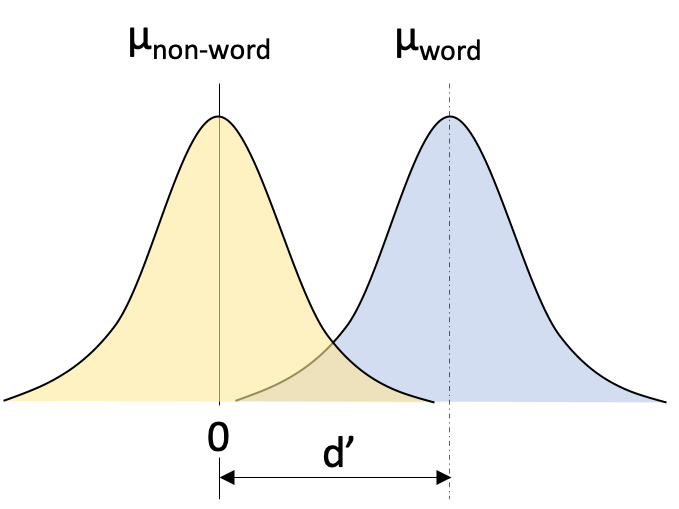
\includegraphics[width=1\linewidth]{SDT_1} \caption{Simple SDT example of lexical decision task}\label{fig:SDT1}
\end{figure}

The second parameter we denote is the criterion (C) parameter. The criterion is the point at which an individual responds non-word (to the left of C in Figure \ref{fig:SDT2}) or word (to the right of C in Figure \ref{fig:SDT2}) and it is set somewhere between the means of the two distributions. If you're biased to respond word, the criterion would move to the left. Conversely, if you're biased to respond non-word then the criterion would move to the right.

\begin{figure}
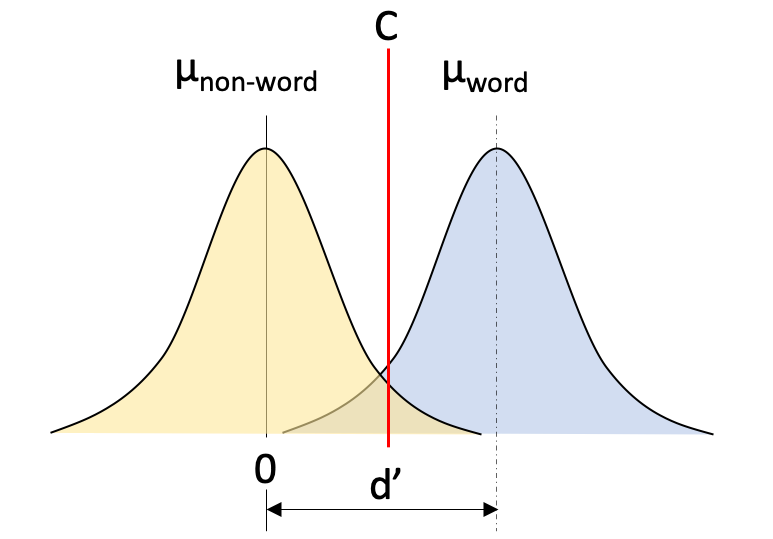
\includegraphics[width=1\linewidth]{SDT_2} \caption{Simple SDT example of lexical decision task}\label{fig:SDT2}
\end{figure}

 Do we need to add something about means should be positive - to the right of NW mean of 0, otherwise the line about ``given these parameters, one would expect that the word distribution would have a higher mean than the non-words, with partial overlap'' does not make sense.

\hypertarget{writing-a-log-likelihood-function}{%
\subsection{Writing a log-likelihood function}\label{writing-a-log-likelihood-function}}

Let's write a simple log likelihood function for a fabricated data set. You can copy the code below to follow along with the example.

\begin{Shaded}
\begin{Highlighting}[]
\NormalTok{resp <-}\StringTok{ }\KeywordTok{c}\NormalTok{(}\StringTok{"word"}\NormalTok{, }\StringTok{"word"}\NormalTok{, }\StringTok{"non-word"}\NormalTok{, }\StringTok{"word"}\NormalTok{, }\StringTok{"non-word"}\NormalTok{, }\StringTok{"non-word"}\NormalTok{, }\StringTok{"word"}\NormalTok{, }\StringTok{"non-word"}\NormalTok{)}
\NormalTok{stim <-}\StringTok{ }\KeywordTok{c}\NormalTok{(}\StringTok{"word"}\NormalTok{, }\StringTok{"word"}\NormalTok{, }\StringTok{"non-word"}\NormalTok{, }\StringTok{"word"}\NormalTok{, }\StringTok{"non-word"}\NormalTok{, }\StringTok{"non-word"}\NormalTok{, }\StringTok{"non-word"}\NormalTok{, }\StringTok{"word"}\NormalTok{)}
\NormalTok{fabData <-}\StringTok{ }\KeywordTok{as.data.frame}\NormalTok{(}\KeywordTok{cbind}\NormalTok{(resp, stim))}
\end{Highlighting}
\end{Shaded}

We create our dataset by combining a response \texttt{resp} and a stimulus \texttt{stim} vector into a data frame as shown in \ref{tab:fakeHead} below.

\begin{table}

\caption{\label{tab:fakeHead}A fabricated dataset of 7 trials with a response and a stimuls column}
\centering
\begin{tabular}[t]{l|l}
\hline
resp & stim\\
\hline
word & word\\
\hline
word & word\\
\hline
non-word & non-word\\
\hline
word & word\\
\hline
non-word & non-word\\
\hline
non-word & non-word\\
\hline
word & non-word\\
\hline
non-word & word\\
\hline
\end{tabular}
\end{table}

Our log likelihood function will step through the data, line by line, and find a likelihood value for each trial, under two parameters; d-prime \texttt{d} and criterion \texttt{C}.

 Remove this paragraph? Some info is covered above
As mentioned \protect\hyperlink{sdtOutline}{above} the non-word distribution has a mean of 0 and SD of 1. This then gives a reference point for where the mean of the word distribution would sit and is denoted by d'.
Now we must find the location of the criterion. Setting the criterion allows us to determine which response will be made i.e.~above the criterion, participant will respond word and below the criterion, participant will respond non-word.

Here is our complete log likelihood function. We have omitted some code from the code blocks below to enhance appearance, so we encourage you to copy the log likelihood function from the following code block if you'd like to follow along with our example.

\begin{Shaded}
\begin{Highlighting}[numbers=left,,]
\NormalTok{SDT_ll <-}\StringTok{ }\ControlFlowTok{function}\NormalTok{(x, data, }\DataTypeTok{sample =} \OtherTok{FALSE}\NormalTok{)\{}
  \ControlFlowTok{if}\NormalTok{ (}\OperatorTok{!}\NormalTok{sample) \{}
\NormalTok{    out <-}\StringTok{ }\KeywordTok{numeric}\NormalTok{(}\KeywordTok{nrow}\NormalTok{(data))}
    \ControlFlowTok{for}\NormalTok{ (i }\ControlFlowTok{in} \DecValTok{1}\OperatorTok{:}\KeywordTok{nrow}\NormalTok{(data)) \{}
      \ControlFlowTok{if}\NormalTok{ (stim[i] }\OperatorTok{==}\StringTok{ "word"}\NormalTok{) \{}
      \ControlFlowTok{if}\NormalTok{ (resp[i] }\OperatorTok{==}\StringTok{ "word"}\NormalTok{) \{}
\NormalTok{        out[i] <-}\StringTok{ }\KeywordTok{pnorm}\NormalTok{(x[}\StringTok{"C"}\NormalTok{], }\DataTypeTok{mean =}\NormalTok{ x[}\StringTok{"d"}\NormalTok{], }\DataTypeTok{sd =} \DecValTok{1}\NormalTok{, }
                        \DataTypeTok{log.p =} \OtherTok{TRUE}\NormalTok{, }\DataTypeTok{lower.tail =} \OtherTok{FALSE}\NormalTok{)}
\NormalTok{      \} }\ControlFlowTok{else}\NormalTok{ \{}
\NormalTok{        out[i] <-}\StringTok{ }\KeywordTok{pnorm}\NormalTok{(x[}\StringTok{"C"}\NormalTok{], }\DataTypeTok{mean =}\NormalTok{ x[}\StringTok{"d"}\NormalTok{], }\DataTypeTok{sd =} \DecValTok{1}\NormalTok{, }
                        \DataTypeTok{log.p =} \OtherTok{TRUE}\NormalTok{, }\DataTypeTok{lower.tail =} \OtherTok{TRUE}\NormalTok{)}
\NormalTok{      \}}
\NormalTok{    \} }\ControlFlowTok{else}\NormalTok{ \{}
      \ControlFlowTok{if}\NormalTok{ (resp[i] }\OperatorTok{==}\StringTok{ "word"}\NormalTok{) \{}
\NormalTok{        out[i] <-}\StringTok{ }\KeywordTok{pnorm}\NormalTok{(x[}\StringTok{"C"}\NormalTok{], }\DataTypeTok{mean =} \DecValTok{0}\NormalTok{, }\DataTypeTok{sd =} \DecValTok{1}\NormalTok{, }
                        \DataTypeTok{log.p =} \OtherTok{TRUE}\NormalTok{, }\DataTypeTok{lower.tail =} \OtherTok{FALSE}\NormalTok{)}
\NormalTok{      \} }\ControlFlowTok{else}\NormalTok{ \{}
\NormalTok{        out[i] <-}\StringTok{ }\KeywordTok{pnorm}\NormalTok{(x[}\StringTok{"C"}\NormalTok{], }\DataTypeTok{mean =} \DecValTok{0}\NormalTok{, }\DataTypeTok{sd =} \DecValTok{1}\NormalTok{, }
                        \DataTypeTok{log.p =} \OtherTok{TRUE}\NormalTok{, }\DataTypeTok{lower.tail =} \OtherTok{TRUE}\NormalTok{)}
\NormalTok{        \}}
\NormalTok{      \}}
\NormalTok{  \}}
  \KeywordTok{sum}\NormalTok{(out)}
\NormalTok{  \}}
\NormalTok{\}}
\end{Highlighting}
\end{Shaded}

We initialise the log likelihood function with three arguments

\begin{Shaded}
\begin{Highlighting}[numbers=left,,]
\NormalTok{SDT_ll <-}\StringTok{ }\ControlFlowTok{function}\NormalTok{(x, data, }\DataTypeTok{sample =} \OtherTok{FALSE}\NormalTok{) \{}
\end{Highlighting}
\end{Shaded}

\begin{itemize}
\tightlist
\item
  \texttt{x} is a named parameter vector (e.g.\texttt{pars})
\item
  \texttt{data} is the dataset
\item
  \texttt{sample\ =} sample values from the posterior distribution (For this simple example, we do not require a \texttt{sample} argument.)
\end{itemize}

The first if statement (line 2) checks if you want to sample, this is used for posterior predictive sampling which we will cover in later chapters. and assigns NAs to your data frames response column. If you're not sampling (like us in this example), you need to create an output vector \texttt{out}. The \texttt{out} vector will contain the log likelihood value for each row/trial in your dataset. Need to explain the \texttt{(sample)} part below

\begin{Shaded}
\begin{Highlighting}[numbers=left,,firstnumber=2,]
  \ControlFlowTok{if}\NormalTok{ (sample) \{}
\NormalTok{    data}\OperatorTok{$}\NormalTok{response <-}\StringTok{ }\OtherTok{NA}
\NormalTok{    \} }\ControlFlowTok{else}\NormalTok{ \{}
\NormalTok{      out <-}\StringTok{ }\KeywordTok{numeric}\NormalTok{(}\KeywordTok{nrow}\NormalTok{(data))}
\NormalTok{      \}}
\end{Highlighting}
\end{Shaded}

From line 9, we check each row in the data set, first considering all trials with word stimuli \texttt{if\ (stim{[}i{]}\ ==\ "word"} (line 10), and assign a likelihood for responding word (line 12-13) or non-word (line 15-16). The word distribution has a mean of \texttt{x{[}"d"{]}} (d-prime parameter) and a decision criterion parameter \texttt{x{[}"C"{]}}. If the response is word, we are considering values ABOVE or to the right of C in \ref{fig:SDT2}, so we set \texttt{lower.tail\ =} to \texttt{FALSE}. If the response is non-word, we look for values BELOW or to the left of C in \ref{fig:SDT2} and we set \texttt{lower.tail\ =} to \texttt{TRUE}. The \texttt{log.p\ =} argument takes the log of all likelihood values when set to \texttt{TRUE}. We do this so we can sum all likelihoods at the end of the log likelihood function.
 Do we need to explain p-norm??

\begin{Shaded}
\begin{Highlighting}[numbers=left,,firstnumber=8,]
  \ControlFlowTok{if}\NormalTok{ (}\OperatorTok{!}\NormalTok{sample) \{}
    \ControlFlowTok{for}\NormalTok{ (i }\ControlFlowTok{in} \DecValTok{1}\OperatorTok{:}\KeywordTok{nrow}\NormalTok{(data)) \{}
      \ControlFlowTok{if}\NormalTok{ (stim[i] }\OperatorTok{==}\StringTok{ "word"}\NormalTok{) \{}
        \ControlFlowTok{if}\NormalTok{ (resp[i] }\OperatorTok{==}\StringTok{ "word"}\NormalTok{) \{}
\NormalTok{          out[i] <-}\StringTok{ }\KeywordTok{pnorm}\NormalTok{(x[}\StringTok{"C"}\NormalTok{], }\DataTypeTok{mean =}\NormalTok{ x[}\StringTok{"d"}\NormalTok{], }\DataTypeTok{sd =} \DecValTok{1}\NormalTok{, }
                         \DataTypeTok{log.p =} \OtherTok{TRUE}\NormalTok{, }\DataTypeTok{lower.tail =} \OtherTok{FALSE}\NormalTok{)}
\NormalTok{    \} }\ControlFlowTok{else}\NormalTok{ \{}
\NormalTok{      out[i] <-}\StringTok{ }\KeywordTok{pnorm}\NormalTok{(x[}\StringTok{"C"}\NormalTok{], }\DataTypeTok{mean =}\NormalTok{ x[}\StringTok{"d"}\NormalTok{], }\DataTypeTok{sd =} \DecValTok{1}\NormalTok{, }
                     \DataTypeTok{log.p =} \OtherTok{TRUE}\NormalTok{, }\DataTypeTok{lower.tail =} \OtherTok{TRUE}\NormalTok{)}
\NormalTok{      \}}
\end{Highlighting}
\end{Shaded}

From the else statement on line 18, we have the function for non-word trials i.e. \texttt{stim{[}i{]}\ ==\ "non-word"}. As can be seen below, the output value \texttt{out{[}i{]}} for these trials is arrived at in a similar manner to the word trials. We set the \texttt{mean} to 0 and the standard deviation \texttt{sd} to 1. If the response is word, we are considering values ABOVE or to the right of C in \ref{fig:SDT2}, so we set \texttt{lower.tail\ =} to \texttt{FALSE}. If the response is non-word, we look for values BELOW or to the left of C in \ref{fig:SDT2} and we set \texttt{lower.tail\ =} to \texttt{TRUE}. Again we want the log of all likelihood values so we set \texttt{log.p\ =\ TRUE}.

\begin{Shaded}
\begin{Highlighting}[numbers=left,,firstnumber=18,]
\ControlFlowTok{else}\NormalTok{ \{}
  \ControlFlowTok{if}\NormalTok{ (resp[i] }\OperatorTok{==}\StringTok{ "word"}\NormalTok{) \{}
\NormalTok{    out[i] <-}\StringTok{ }\KeywordTok{pnorm}\NormalTok{(x[}\StringTok{"C"}\NormalTok{], }\DataTypeTok{mean =} \DecValTok{0}\NormalTok{, }\DataTypeTok{sd =} \DecValTok{1}\NormalTok{, }
                    \DataTypeTok{log.p =} \OtherTok{TRUE}\NormalTok{, }\DataTypeTok{lower.tail =} \OtherTok{FALSE}\NormalTok{)}
\NormalTok{        \} }\ControlFlowTok{else}\NormalTok{ \{}
\NormalTok{          out[i] <-}\StringTok{ }\KeywordTok{pnorm}\NormalTok{(x[}\StringTok{"C"}\NormalTok{], }\DataTypeTok{mean =} \DecValTok{0}\NormalTok{, }\DataTypeTok{sd =} \DecValTok{1}\NormalTok{, }
                         \DataTypeTok{log.p =} \OtherTok{TRUE}\NormalTok{, }\DataTypeTok{lower.tail =} \OtherTok{TRUE}\NormalTok{)}
\NormalTok{        \}}
\NormalTok{      \}}
\end{Highlighting}
\end{Shaded}

The final line of code on line 24 sums the \texttt{out} vector and returns a log-likelihood value for your model.
 The text alignment/justification for code blocks is determined by the length of the longest line in the code block

\begin{Shaded}
\begin{Highlighting}[]
\KeywordTok{sum}\NormalTok{(out)}
\end{Highlighting}
\end{Shaded}

\hypertarget{testing-the-sdt-log-likelihood-function}{%
\section{Testing the SDT log likelihood function}\label{testing-the-sdt-log-likelihood-function}}

Before we run the log likelihood function, we must create a parameter vector \texttt{pars} containing the same parameter names used in our log likelihood function above i.e.~we name the criterion \texttt{C} and d-prime parameter \texttt{d} and we assign arbitrary values to each parameter.

\begin{Shaded}
\begin{Highlighting}[]
\NormalTok{pars <-}\StringTok{ }\KeywordTok{c}\NormalTok{(}\DataTypeTok{C =} \FloatTok{0.8}\NormalTok{, }\DataTypeTok{d =} \DecValTok{2}\NormalTok{)}
\end{Highlighting}
\end{Shaded}

We can test run our log likelihood function by passing in the parameter vector \texttt{pars} and the fabricated dataset we created above \texttt{fabData}.

\begin{Shaded}
\begin{Highlighting}[]
\KeywordTok{SDT_loglike}\NormalTok{(pars, fabData)}
\end{Highlighting}
\end{Shaded}

\begin{verbatim}
## [1] -4.795029
\end{verbatim}

Now, if we change the parameter values, the log-likelihood value should also change.

\begin{Shaded}
\begin{Highlighting}[]
\NormalTok{pars <-}\StringTok{ }\KeywordTok{replace}\NormalTok{(pars, }\KeywordTok{c}\NormalTok{(}\DecValTok{1}\NormalTok{,}\DecValTok{2}\NormalTok{), }\KeywordTok{c}\NormalTok{(}\FloatTok{0.5}\NormalTok{, }\FloatTok{1.2}\NormalTok{))}
\KeywordTok{SDT_loglike}\NormalTok{(pars, fabData)}
\end{Highlighting}
\end{Shaded}

\begin{verbatim}
## [1] -4.532791
\end{verbatim}

We can see the log likelihood has changed, so these values are more accurate given the data.
 What does this tell us? Seems insufficient to look for a change in the LL

\hypertarget{sdt-log-likelihood-function-for-wagenmakers-experiment}{%
\section{SDT log likelihood function for Wagenmakers experiment}\label{sdt-log-likelihood-function-for-wagenmakers-experiment}}

Now that we've covered a simple test example, let's create a log likelihood function for the \citet{wagenmakers2008diffusion} dataset.

\hypertarget{description-of-wagenmakers-experiment}{%
\subsection{Description of Wagenmakers experiment}\label{description-of-wagenmakers-experiment}}

If you'd like to follow our example, you will need to access the Wagenmakers dataset. This can be done by installing the \texttt{rtdists} package and calling the \texttt{speed\_acc} data frame. The structure of the \texttt{speed\_acc} dataset will need to be modified in order to meet the requirements of the PMwG sampler. To do this, modify the dataset to match the structure illustrated in table \ref{tab:wagenmakers10}.

Participants were asked to indicate whether a letter string was a word or a non-word. A subset of Wagenmaker et al data are shown in table \ref{tab:wagenmakers10}, with each line representing a single trial. We have a \texttt{subject} column with a subject id (1-19), a condition column \texttt{cond} which indicates the proportion of words to non-words presented within a block of trials. In word blocks (\texttt{cond\ =\ w}) participants completed 75\% word and 25\% non-word trials and for non-word (\texttt{cond\ =\ nw}) blocks 75\% non-word and 25\% word trials. The \texttt{stim} column lists the word's frequency i.e.~is the stimulus a very low frequency word (\texttt{stim\ =\ vlf}), a low frequency word (\texttt{stim\ =\ lf}), a high frequency word (\texttt{stim\ =\ hf}) or a non-word (\texttt{stim\ =\ nw}). The third column \texttt{resp} refers to the participant's response i.e.~the participant responded word (\texttt{resp\ =\ W}) or non-word (\texttt{resp\ =\ NW}). The two remaining columns list the response time (\texttt{rt}) and whether the paricipant made a correct (\texttt{correct\ =\ 2}) or incorrect (\texttt{correct\ =\ 1}) choice. For more details about the experiment please see \href{https://www.sciencedirect.com/science/article/pii/S0749596X07000496}{the original paper}. Is this the correct paper to reference?

\begin{table}

\caption{\label{tab:wagenmakers10}Subset of 10 trials from the Wagenmakers (2008) dataset.}
\centering
\begin{tabular}[t]{r|l|l|l|r|r}
\hline
subject & cond & stim & resp & rt & correct\\
\hline
1 & w & lf & W & 0.410 & 2\\
\hline
1 & w & hf & W & 0.426 & 2\\
\hline
1 & w & nw & NW & 0.499 & 2\\
\hline
1 & w & lf & W & 0.392 & 2\\
\hline
1 & w & vlf & W & 0.435 & 2\\
\hline
1 & w & hf & W & 0.376 & 2\\
\hline
1 & nw & lf & W & 0.861 & 2\\
\hline
1 & nw & hf & W & 0.563 & 2\\
\hline
1 & nw & nw & NW & 0.666 & 2\\
\hline
1 & nw & nw & NW & 1.561 & 2\\
\hline
1 & nw & nw & NW & 0.503 & 2\\
\hline
1 & nw & nw & NW & 0.445 & 2\\
\hline
\end{tabular}
\end{table}

Our log-likelihood function for Wagenmakers experimental data is similar to the function we wrote above, except now we require a criterion parameter for each condition and a d-prime parameter for each of the \texttt{stim} word types. This is illustrated in figure \ref{fig:SDT3} below, where we have a non-word criterion Cnw, a word criterion Cw and three distributions for each of the \texttt{stim} types with corresponding d-prime for each distribution: dvlf, dlf, dhf.

\begin{figure}
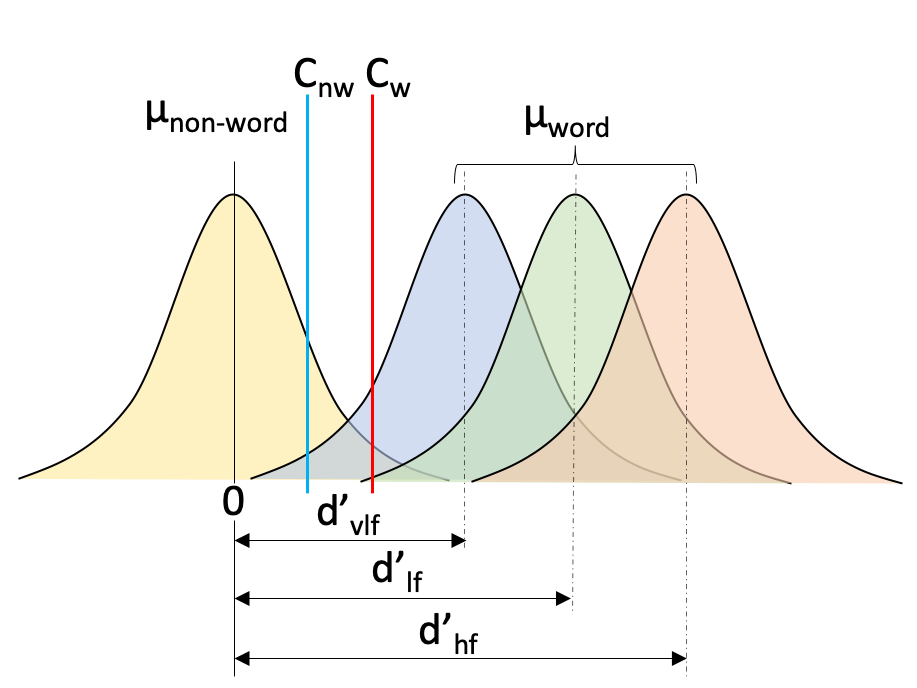
\includegraphics[width=1\linewidth]{SDT_3} \caption{Signal detection theory example of lexical decision task}\label{fig:SDT3}
\end{figure}

Here is our complete log likelihood function for the Wagenmakers data set.

\begin{Shaded}
\begin{Highlighting}[numbers=left,,]
\NormalTok{SDT_ll <-}\StringTok{ }\ControlFlowTok{function}\NormalTok{(x, data, }\DataTypeTok{sample=}\OtherTok{FALSE}\NormalTok{)\{}
  \ControlFlowTok{if}\NormalTok{ (sample)\{}
\NormalTok{    data}\OperatorTok{$}\NormalTok{response <-}\StringTok{ }\OtherTok{NA}
\NormalTok{  \} }\ControlFlowTok{else}\NormalTok{ \{}
\NormalTok{    out <-}\StringTok{ }\KeywordTok{numeric}\NormalTok{(}\KeywordTok{nrow}\NormalTok{(data))}
\NormalTok{  \}}
  \ControlFlowTok{if}\NormalTok{ (}\OperatorTok{!}\NormalTok{sample)\{}
  \ControlFlowTok{for}\NormalTok{ (i }\ControlFlowTok{in} \DecValTok{1}\OperatorTok{:}\KeywordTok{nrow}\NormalTok{(data)) \{}
    \ControlFlowTok{if}\NormalTok{ (data}\OperatorTok{$}\NormalTok{cond[i] }\OperatorTok{==}\StringTok{ "w"}\NormalTok{) \{}
    \ControlFlowTok{if}\NormalTok{ (data}\OperatorTok{$}\NormalTok{stim[i] }\OperatorTok{==}\StringTok{ "hf"}\NormalTok{) \{}
      \ControlFlowTok{if}\NormalTok{ (data}\OperatorTok{$}\NormalTok{resp[i] }\OperatorTok{==}\StringTok{ "W"}\NormalTok{) \{}
\NormalTok{        out[i] <-}\StringTok{ }\KeywordTok{pnorm}\NormalTok{(x[}\StringTok{"C.w"}\NormalTok{], }\DataTypeTok{mean =}\NormalTok{ x[}\StringTok{"HF.d"}\NormalTok{], }\DataTypeTok{sd =} \DecValTok{1}\NormalTok{,}
                       \DataTypeTok{log.p =} \OtherTok{TRUE}\NormalTok{, }\DataTypeTok{lower.tail =} \OtherTok{FALSE}\NormalTok{)}
\NormalTok{      \} }\ControlFlowTok{else}\NormalTok{ \{}
\NormalTok{        out[i] <-}\StringTok{ }\KeywordTok{pnorm}\NormalTok{(x[}\StringTok{"C.w"}\NormalTok{], }\DataTypeTok{mean =}\NormalTok{ x[}\StringTok{"HF.d"}\NormalTok{], }\DataTypeTok{sd =} \DecValTok{1}\NormalTok{,}
                       \DataTypeTok{log.p =} \OtherTok{TRUE}\NormalTok{, }\DataTypeTok{lower.tail =} \OtherTok{TRUE}\NormalTok{)}
\NormalTok{      \}}
\NormalTok{    \} }\ControlFlowTok{else} \ControlFlowTok{if}\NormalTok{ (data}\OperatorTok{$}\NormalTok{stim[i] }\OperatorTok{==}\StringTok{ "lf"}\NormalTok{)\{}
      \ControlFlowTok{if}\NormalTok{ (data}\OperatorTok{$}\NormalTok{resp[i] }\OperatorTok{==}\StringTok{ "W"}\NormalTok{)\{}
\NormalTok{        out[i] <-}\StringTok{ }\KeywordTok{pnorm}\NormalTok{(x[}\StringTok{"C.w"}\NormalTok{], }\DataTypeTok{mean =}\NormalTok{ x[}\StringTok{"LF.d"}\NormalTok{], }\DataTypeTok{sd =} \DecValTok{1}\NormalTok{,}
                       \DataTypeTok{log.p =} \OtherTok{TRUE}\NormalTok{, }\DataTypeTok{lower.tail =} \OtherTok{FALSE}\NormalTok{)}
\NormalTok{      \} }\ControlFlowTok{else}\NormalTok{ \{}
\NormalTok{        out[i] <-}\StringTok{ }\KeywordTok{pnorm}\NormalTok{(x[}\StringTok{"C.w"}\NormalTok{], }\DataTypeTok{mean =}\NormalTok{ x[}\StringTok{"LF.d"}\NormalTok{], }\DataTypeTok{sd =} \DecValTok{1}\NormalTok{,}
                       \DataTypeTok{log.p =} \OtherTok{TRUE}\NormalTok{, }\DataTypeTok{lower.tail =} \OtherTok{TRUE}\NormalTok{)}
\NormalTok{        \}}
\NormalTok{      \} }\ControlFlowTok{else} \ControlFlowTok{if}\NormalTok{ (data}\OperatorTok{$}\NormalTok{stim[i] }\OperatorTok{==}\StringTok{ "vlf"}\NormalTok{) \{}
        \ControlFlowTok{if}\NormalTok{ (data}\OperatorTok{$}\NormalTok{resp[i] }\OperatorTok{==}\StringTok{ "W"}\NormalTok{) \{}
\NormalTok{          out[i] <-}\StringTok{ }\KeywordTok{pnorm}\NormalTok{(x[}\StringTok{"C.w"}\NormalTok{], }\DataTypeTok{mean =}\NormalTok{ x[}\StringTok{"VLF.d"}\NormalTok{], }\DataTypeTok{sd =} \DecValTok{1}\NormalTok{,}
                         \DataTypeTok{log.p =} \OtherTok{TRUE}\NormalTok{, }\DataTypeTok{lower.tail =} \OtherTok{FALSE}\NormalTok{)}
\NormalTok{        \} }\ControlFlowTok{else}\NormalTok{ \{}
\NormalTok{          out[i] <-}\StringTok{ }\KeywordTok{pnorm}\NormalTok{(x[}\StringTok{"C.w"}\NormalTok{], }\DataTypeTok{mean =}\NormalTok{ x[}\StringTok{"VLF.d"}\NormalTok{], }\DataTypeTok{sd =} \DecValTok{1}\NormalTok{,}
                         \DataTypeTok{log.p =} \OtherTok{TRUE}\NormalTok{, }\DataTypeTok{lower.tail =} \OtherTok{TRUE}\NormalTok{)}
\NormalTok{          \}}
\NormalTok{        \} }\ControlFlowTok{else}\NormalTok{ \{}
      \ControlFlowTok{if}\NormalTok{ (data}\OperatorTok{$}\NormalTok{resp[i] }\OperatorTok{==}\StringTok{ "W"}\NormalTok{) \{}
\NormalTok{        out[i] <-}\StringTok{ }\KeywordTok{pnorm}\NormalTok{(x[}\StringTok{"C.w"}\NormalTok{], }\DataTypeTok{mean =} \DecValTok{0}\NormalTok{, }\DataTypeTok{sd =} \DecValTok{1}\NormalTok{,}
                       \DataTypeTok{log.p =} \OtherTok{TRUE}\NormalTok{, }\DataTypeTok{lower.tail =} \OtherTok{FALSE}\NormalTok{)}
\NormalTok{      \} }\ControlFlowTok{else}\NormalTok{ \{}
\NormalTok{        out[i] <-}\StringTok{ }\KeywordTok{pnorm}\NormalTok{(x[}\StringTok{"C.w"}\NormalTok{], }\DataTypeTok{mean =} \DecValTok{0}\NormalTok{, }\DataTypeTok{sd =} \DecValTok{1}\NormalTok{,}
                       \DataTypeTok{log.p =} \OtherTok{TRUE}\NormalTok{, }\DataTypeTok{lower.tail =} \OtherTok{TRUE}\NormalTok{)}
\NormalTok{        \}}
\NormalTok{      \}}
\NormalTok{    \} }\ControlFlowTok{else}\NormalTok{ \{}
      \ControlFlowTok{if}\NormalTok{ (data}\OperatorTok{$}\NormalTok{stim[i] }\OperatorTok{==}\StringTok{ "hf"}\NormalTok{) \{}
        \ControlFlowTok{if}\NormalTok{ (data}\OperatorTok{$}\NormalTok{resp[i] }\OperatorTok{==}\StringTok{ "W"}\NormalTok{) \{}
\NormalTok{          out[i] <-}\StringTok{ }\KeywordTok{pnorm}\NormalTok{(x[}\StringTok{"C.nw"}\NormalTok{], }\DataTypeTok{mean =}\NormalTok{ x[}\StringTok{"HF.d"}\NormalTok{], }\DataTypeTok{sd =} \DecValTok{1}\NormalTok{, }
                         \DataTypeTok{log.p =} \OtherTok{TRUE}\NormalTok{, }\DataTypeTok{lower.tail =} \OtherTok{FALSE}\NormalTok{)}
\NormalTok{        \} }\ControlFlowTok{else}\NormalTok{ \{}
\NormalTok{          out[i] <-}\StringTok{ }\KeywordTok{pnorm}\NormalTok{(x[}\StringTok{"C.nw"}\NormalTok{], }\DataTypeTok{mean =}\NormalTok{ x[}\StringTok{"HF.d"}\NormalTok{], }\DataTypeTok{sd =} \DecValTok{1}\NormalTok{, }
                         \DataTypeTok{log.p =} \OtherTok{TRUE}\NormalTok{, }\DataTypeTok{lower.tail =} \OtherTok{TRUE}\NormalTok{)}
\NormalTok{        \}}
\NormalTok{      \}  }\ControlFlowTok{else} \ControlFlowTok{if}\NormalTok{ (data}\OperatorTok{$}\NormalTok{stim[i] }\OperatorTok{==}\StringTok{ "lf"}\NormalTok{) \{}
        \ControlFlowTok{if}\NormalTok{ (data}\OperatorTok{$}\NormalTok{resp[i] }\OperatorTok{==}\StringTok{ "W"}\NormalTok{) \{}
\NormalTok{          out[i] <-}\StringTok{ }\KeywordTok{pnorm}\NormalTok{(x[}\StringTok{"C.nw"}\NormalTok{], }\DataTypeTok{mean =}\NormalTok{ x[}\StringTok{"LF.d"}\NormalTok{], }\DataTypeTok{sd =} \DecValTok{1}\NormalTok{, }
                         \DataTypeTok{log.p =} \OtherTok{TRUE}\NormalTok{, }\DataTypeTok{lower.tail =} \OtherTok{FALSE}\NormalTok{)}
\NormalTok{        \} }\ControlFlowTok{else}\NormalTok{ \{}
\NormalTok{          out[i] <-}\StringTok{ }\KeywordTok{pnorm}\NormalTok{(x[}\StringTok{"C.nw"}\NormalTok{], }\DataTypeTok{mean =}\NormalTok{ x[}\StringTok{"LF.d"}\NormalTok{], }\DataTypeTok{sd =} \DecValTok{1}\NormalTok{, }
                         \DataTypeTok{log.p =} \OtherTok{TRUE}\NormalTok{, }\DataTypeTok{lower.tail =} \OtherTok{TRUE}\NormalTok{)}
\NormalTok{        \}}
\NormalTok{      \} }\ControlFlowTok{else} \ControlFlowTok{if}\NormalTok{ (data}\OperatorTok{$}\NormalTok{stim[i] }\OperatorTok{==}\StringTok{ "vlf"}\NormalTok{) \{}
        \ControlFlowTok{if}\NormalTok{ (data}\OperatorTok{$}\NormalTok{resp[i] }\OperatorTok{==}\StringTok{ "W"}\NormalTok{) \{}
\NormalTok{          out[i] <-}\StringTok{ }\KeywordTok{pnorm}\NormalTok{(x[}\StringTok{"C.nw"}\NormalTok{], }\DataTypeTok{mean =}\NormalTok{ x[}\StringTok{"VLF.d"}\NormalTok{], }\DataTypeTok{sd =} \DecValTok{1}\NormalTok{, }
                         \DataTypeTok{log.p =} \OtherTok{TRUE}\NormalTok{, }\DataTypeTok{lower.tail =} \OtherTok{FALSE}\NormalTok{)}
\NormalTok{        \} }\ControlFlowTok{else}\NormalTok{ \{}
\NormalTok{          out[i] <-}\StringTok{ }\KeywordTok{pnorm}\NormalTok{(x[}\StringTok{"C.nw"}\NormalTok{], }\DataTypeTok{mean =}\NormalTok{ x[}\StringTok{"VLF.d"}\NormalTok{], }\DataTypeTok{sd =} \DecValTok{1}\NormalTok{, }
                         \DataTypeTok{log.p =} \OtherTok{TRUE}\NormalTok{, }\DataTypeTok{lower.tail =} \OtherTok{TRUE}\NormalTok{)}
\NormalTok{        \}}
\NormalTok{      \} }\ControlFlowTok{else}\NormalTok{ \{}
        \ControlFlowTok{if}\NormalTok{ (data}\OperatorTok{$}\NormalTok{resp[i] }\OperatorTok{==}\StringTok{ "W"}\NormalTok{) \{}
\NormalTok{          out[i] <-}\StringTok{ }\KeywordTok{pnorm}\NormalTok{(x[}\StringTok{"C.nw"}\NormalTok{], }\DataTypeTok{mean =} \DecValTok{0}\NormalTok{, }\DataTypeTok{sd =} \DecValTok{1}\NormalTok{, }
                         \DataTypeTok{log.p =} \OtherTok{TRUE}\NormalTok{, }\DataTypeTok{lower.tail =} \OtherTok{FALSE}\NormalTok{)}
\NormalTok{        \} }\ControlFlowTok{else}\NormalTok{ \{}
\NormalTok{          out[i] <-}\StringTok{ }\KeywordTok{pnorm}\NormalTok{(x[}\StringTok{"C.nw"}\NormalTok{], }\DataTypeTok{mean =} \DecValTok{0}\NormalTok{, }\DataTypeTok{sd =} \DecValTok{1}\NormalTok{, }
                         \DataTypeTok{log.p =} \OtherTok{TRUE}\NormalTok{, }\DataTypeTok{lower.tail =} \OtherTok{TRUE}\NormalTok{)}
\NormalTok{        \}}
\NormalTok{      \}}
\NormalTok{    \}}
\NormalTok{  \}}
  \KeywordTok{sum}\NormalTok{(out)}
\NormalTok{  \}}
\NormalTok{\}}
\end{Highlighting}
\end{Shaded}

Line 1 through to line 8 are the same as the log likelihood we wrote for the fabricated dataset above. From line 9, we calculate the log-likelihood \texttt{out{[}i{]}} for word condition trials \texttt{cond{[}i{]}\ ==\ "w"} when the stimulus is a high frequency word \texttt{stim{[}i{]}\ ==\ "hf"} for each response. We do this by considering the upper tail of the high frequency word distribution \texttt{lower.tail\ =\ FALSE}, from the word criterion Cw, for word responses \texttt{resp{[}i{]}\ ==\ "W"} and the lower tail for non-word responses (\texttt{else} statement on line 14).

\begin{Shaded}
\begin{Highlighting}[numbers=left,,firstnumber=9,]
 \ControlFlowTok{if}\NormalTok{ (data}\OperatorTok{$}\NormalTok{cond[i] }\OperatorTok{==}\StringTok{ "w"}\NormalTok{) \{}
    \ControlFlowTok{if}\NormalTok{ (data}\OperatorTok{$}\NormalTok{stim[i] }\OperatorTok{==}\StringTok{ "hf"}\NormalTok{) \{}
      \ControlFlowTok{if}\NormalTok{ (data}\OperatorTok{$}\NormalTok{resp[i] }\OperatorTok{==}\StringTok{ "W"}\NormalTok{) \{}
\NormalTok{        out[i] <-}\StringTok{ }\KeywordTok{pnorm}\NormalTok{(x[}\StringTok{"C.w"}\NormalTok{], }\DataTypeTok{mean =}\NormalTok{ x[}\StringTok{"HF.d"}\NormalTok{], }\DataTypeTok{sd =} \DecValTok{1}\NormalTok{,}
                       \DataTypeTok{log.p =} \OtherTok{TRUE}\NormalTok{, }\DataTypeTok{lower.tail =} \OtherTok{FALSE}\NormalTok{)}
\NormalTok{      \} }\ControlFlowTok{else}\NormalTok{ \{}
\NormalTok{        out[i] <-}\StringTok{ }\KeywordTok{pnorm}\NormalTok{(x[}\StringTok{"C.w"}\NormalTok{], }\DataTypeTok{mean =}\NormalTok{ x[}\StringTok{"HF.d"}\NormalTok{], }\DataTypeTok{sd =} \DecValTok{1}\NormalTok{,}
                       \DataTypeTok{log.p =} \OtherTok{TRUE}\NormalTok{, }\DataTypeTok{lower.tail =} \OtherTok{TRUE}\NormalTok{)}
\NormalTok{      \}}
\end{Highlighting}
\end{Shaded}

From line 18 and still considering trials from the word condition, we calculate the log likelihood for each response for low frequency words \texttt{stim{[}i{]}\ ==\ "lf"}, very low frequency words \texttt{stim{[}i{]}\ ==\ "vlf"} (line 26) and non-word stimuli (\texttt{else} statement on line 35).

\begin{Shaded}
\begin{Highlighting}[numbers=left,,firstnumber=18,]
  \ControlFlowTok{else} \ControlFlowTok{if}\NormalTok{ (data}\OperatorTok{$}\NormalTok{stim[i] }\OperatorTok{==}\StringTok{ "lf"}\NormalTok{) \{}
      \ControlFlowTok{if}\NormalTok{ (data}\OperatorTok{$}\NormalTok{resp[i] }\OperatorTok{==}\StringTok{ "W"}\NormalTok{) \{}
\NormalTok{        out[i] <-}\StringTok{ }\KeywordTok{pnorm}\NormalTok{(x[}\StringTok{"C.w"}\NormalTok{], }\DataTypeTok{mean =}\NormalTok{ x[}\StringTok{"LF.d"}\NormalTok{], }\DataTypeTok{sd =} \DecValTok{1}\NormalTok{,}
                       \DataTypeTok{log.p =} \OtherTok{TRUE}\NormalTok{, }\DataTypeTok{lower.tail =} \OtherTok{FALSE}\NormalTok{)}
\NormalTok{      \} }\ControlFlowTok{else}\NormalTok{ \{}
\NormalTok{        out[i] <-}\StringTok{ }\KeywordTok{pnorm}\NormalTok{(x[}\StringTok{"C.w"}\NormalTok{], }\DataTypeTok{mean =}\NormalTok{ x[}\StringTok{"LF.d"}\NormalTok{], }\DataTypeTok{sd =} \DecValTok{1}\NormalTok{,}
                       \DataTypeTok{log.p =} \OtherTok{TRUE}\NormalTok{, }\DataTypeTok{lower.tail =} \OtherTok{TRUE}\NormalTok{)}
\NormalTok{        \}}
\NormalTok{      \} }\ControlFlowTok{else} \ControlFlowTok{if}\NormalTok{ (data}\OperatorTok{$}\NormalTok{stim[i] }\OperatorTok{==}\StringTok{ "vlf"}\NormalTok{) \{}
        \ControlFlowTok{if}\NormalTok{ (data}\OperatorTok{$}\NormalTok{resp[i] }\OperatorTok{==}\StringTok{ "W"}\NormalTok{) \{}
\NormalTok{          out[i] <-}\StringTok{ }\KeywordTok{pnorm}\NormalTok{(x[}\StringTok{"C.w"}\NormalTok{], }\DataTypeTok{mean =}\NormalTok{ x[}\StringTok{"VLF.d"}\NormalTok{], }\DataTypeTok{sd =} \DecValTok{1}\NormalTok{,}
                         \DataTypeTok{log.p =} \OtherTok{TRUE}\NormalTok{, }\DataTypeTok{lower.tail =} \OtherTok{FALSE}\NormalTok{)}
\NormalTok{        \} }\ControlFlowTok{else}\NormalTok{ \{}
\NormalTok{          out[i] <-}\StringTok{ }\KeywordTok{pnorm}\NormalTok{(x[}\StringTok{"C.w"}\NormalTok{], }\DataTypeTok{mean =}\NormalTok{ x[}\StringTok{"VLF.d"}\NormalTok{], }\DataTypeTok{sd =} \DecValTok{1}\NormalTok{,}
                         \DataTypeTok{log.p =} \OtherTok{TRUE}\NormalTok{, }\DataTypeTok{lower.tail =} \OtherTok{TRUE}\NormalTok{)}
\NormalTok{          \}}
\NormalTok{        \} }\ControlFlowTok{else}\NormalTok{ \{}
      \ControlFlowTok{if}\NormalTok{ (data}\OperatorTok{$}\NormalTok{resp[i] }\OperatorTok{==}\StringTok{ "W"}\NormalTok{) \{}
\NormalTok{        out[i] <-}\StringTok{ }\KeywordTok{pnorm}\NormalTok{(x[}\StringTok{"C.w"}\NormalTok{], }\DataTypeTok{mean =} \DecValTok{0}\NormalTok{, }\DataTypeTok{sd =} \DecValTok{1}\NormalTok{,}
                       \DataTypeTok{log.p =} \OtherTok{TRUE}\NormalTok{, }\DataTypeTok{lower.tail =} \OtherTok{FALSE}\NormalTok{)}
\NormalTok{      \} }\ControlFlowTok{else}\NormalTok{ \{}
\NormalTok{        out[i] <-}\StringTok{ }\KeywordTok{pnorm}\NormalTok{(x[}\StringTok{"C.w"}\NormalTok{], }\DataTypeTok{mean =} \DecValTok{0}\NormalTok{, }\DataTypeTok{sd =} \DecValTok{1}\NormalTok{,}
                       \DataTypeTok{log.p =} \OtherTok{TRUE}\NormalTok{, }\DataTypeTok{lower.tail =} \OtherTok{TRUE}\NormalTok{)}
\NormalTok{        \}}
\NormalTok{      \}}
\end{Highlighting}
\end{Shaded}

That covers the word condition. From line 45 through 78, we repeat the same process for the non-word conditon\ldots{}.

\begin{Shaded}
\begin{Highlighting}[numbers=left,,firstnumber=45,]
\ControlFlowTok{else}\NormalTok{ \{}
      \ControlFlowTok{if}\NormalTok{ (data}\OperatorTok{$}\NormalTok{stim[i] }\OperatorTok{==}\StringTok{ "hf"}\NormalTok{) \{}
        \ControlFlowTok{if}\NormalTok{ (data}\OperatorTok{$}\NormalTok{resp[i] }\OperatorTok{==}\StringTok{ "W"}\NormalTok{) \{}
\NormalTok{          out[i] <-}\StringTok{ }\KeywordTok{pnorm}\NormalTok{(x[}\StringTok{"C.nw"}\NormalTok{], }\DataTypeTok{mean =}\NormalTok{ x[}\StringTok{"HF.d"}\NormalTok{], }\DataTypeTok{sd =} \DecValTok{1}\NormalTok{, }
                         \DataTypeTok{log.p =} \OtherTok{TRUE}\NormalTok{, }\DataTypeTok{lower.tail =} \OtherTok{FALSE}\NormalTok{)}
\NormalTok{        \} }\ControlFlowTok{else}\NormalTok{ \{}
\NormalTok{          out[i] <-}\StringTok{ }\KeywordTok{pnorm}\NormalTok{(x[}\StringTok{"C.nw"}\NormalTok{], }\DataTypeTok{mean =}\NormalTok{ x[}\StringTok{"HF.d"}\NormalTok{], }\DataTypeTok{sd =} \DecValTok{1}\NormalTok{, }
                         \DataTypeTok{log.p =} \OtherTok{TRUE}\NormalTok{, }\DataTypeTok{lower.tail =} \OtherTok{TRUE}\NormalTok{)}
\NormalTok{        \}}
\NormalTok{      \} }\ControlFlowTok{else} \ControlFlowTok{if}\NormalTok{ (data}\OperatorTok{$}\NormalTok{stim[i] }\OperatorTok{==}\StringTok{ "lf"}\NormalTok{) \{}
        \ControlFlowTok{if}\NormalTok{ (data}\OperatorTok{$}\NormalTok{resp[i] }\OperatorTok{==}\StringTok{ "W"}\NormalTok{) \{}
\NormalTok{          out[i] <-}\StringTok{ }\KeywordTok{pnorm}\NormalTok{(x[}\StringTok{"C.nw"}\NormalTok{], }\DataTypeTok{mean =}\NormalTok{ x[}\StringTok{"LF.d"}\NormalTok{], }\DataTypeTok{sd =} \DecValTok{1}\NormalTok{, }
                         \DataTypeTok{log.p =} \OtherTok{TRUE}\NormalTok{, }\DataTypeTok{lower.tail =} \OtherTok{FALSE}\NormalTok{)}
\NormalTok{        \} }\ControlFlowTok{else}\NormalTok{ \{}
\NormalTok{          out[i] <-}\StringTok{ }\KeywordTok{pnorm}\NormalTok{(x[}\StringTok{"C.nw"}\NormalTok{], }\DataTypeTok{mean =}\NormalTok{ x[}\StringTok{"LF.d"}\NormalTok{], }\DataTypeTok{sd =} \DecValTok{1}\NormalTok{, }
                         \DataTypeTok{log.p =} \OtherTok{TRUE}\NormalTok{, }\DataTypeTok{lower.tail =} \OtherTok{TRUE}\NormalTok{)}
\NormalTok{        \}}
\NormalTok{      \} }\ControlFlowTok{else} \ControlFlowTok{if}\NormalTok{ (data}\OperatorTok{$}\NormalTok{stim[i] }\OperatorTok{==}\StringTok{ "vlf"}\NormalTok{) \{}
        \ControlFlowTok{if}\NormalTok{ (data}\OperatorTok{$}\NormalTok{resp[i] }\OperatorTok{==}\StringTok{ "W"}\NormalTok{) \{}
\NormalTok{          out[i] <-}\StringTok{ }\KeywordTok{pnorm}\NormalTok{(x[}\StringTok{"C.nw"}\NormalTok{], }\DataTypeTok{mean =}\NormalTok{ x[}\StringTok{"VLF.d"}\NormalTok{], }\DataTypeTok{sd =} \DecValTok{1}\NormalTok{, }
                         \DataTypeTok{log.p =} \OtherTok{TRUE}\NormalTok{, }\DataTypeTok{lower.tail =} \OtherTok{FALSE}\NormalTok{)}
\NormalTok{        \} }\ControlFlowTok{else}\NormalTok{ \{}
\NormalTok{          out[i] <-}\StringTok{ }\KeywordTok{pnorm}\NormalTok{(x[}\StringTok{"C.nw"}\NormalTok{], }\DataTypeTok{mean =}\NormalTok{ x[}\StringTok{"VLF.d"}\NormalTok{], }\DataTypeTok{sd =} \DecValTok{1}\NormalTok{, }
                         \DataTypeTok{log.p =} \OtherTok{TRUE}\NormalTok{, }\DataTypeTok{lower.tail =} \OtherTok{TRUE}\NormalTok{)}
\NormalTok{        \}}
\NormalTok{      \} }\ControlFlowTok{else}\NormalTok{ \{}
        \ControlFlowTok{if}\NormalTok{ (data}\OperatorTok{$}\NormalTok{resp[i] }\OperatorTok{==}\StringTok{ "W"}\NormalTok{) \{}
\NormalTok{          out[i] <-}\StringTok{ }\KeywordTok{pnorm}\NormalTok{(x[}\StringTok{"C.nw"}\NormalTok{], }\DataTypeTok{mean =} \DecValTok{0}\NormalTok{, }\DataTypeTok{sd =} \DecValTok{1}\NormalTok{, }
                         \DataTypeTok{log.p =} \OtherTok{TRUE}\NormalTok{, }\DataTypeTok{lower.tail =} \OtherTok{FALSE}\NormalTok{)}
\NormalTok{        \} }\ControlFlowTok{else}\NormalTok{ \{}
\NormalTok{          out[i] <-}\StringTok{ }\KeywordTok{pnorm}\NormalTok{(x[}\StringTok{"C.nw"}\NormalTok{], }\DataTypeTok{mean =} \DecValTok{0}\NormalTok{, }\DataTypeTok{sd =} \DecValTok{1}\NormalTok{, }
                         \DataTypeTok{log.p =} \OtherTok{TRUE}\NormalTok{, }\DataTypeTok{lower.tail =} \OtherTok{TRUE}\NormalTok{)}
\NormalTok{        \}}
\end{Highlighting}
\end{Shaded}

\ldots{}and sum the values and return the log-likelihood for our model.

\begin{Shaded}
\begin{Highlighting}[]
  \KeywordTok{sum}\NormalTok{(out)}
\end{Highlighting}
\end{Shaded}

This give us a log likelihood for all data. Let's test this\ldots{}

\begin{Shaded}
\begin{Highlighting}[]
\NormalTok{pars <-}\StringTok{ }\KeywordTok{log}\NormalTok{(}\KeywordTok{c}\NormalTok{(}\DataTypeTok{C.w =} \DecValTok{1}\NormalTok{, }\DataTypeTok{C.nw =} \FloatTok{0.5}\NormalTok{, }\DataTypeTok{HF.d =} \DecValTok{3}\NormalTok{, }\DataTypeTok{LF.d =} \FloatTok{1.8}\NormalTok{, }\DataTypeTok{VLF.d =} \FloatTok{0.7}\NormalTok{))}
\KeywordTok{SDT_ll}\NormalTok{(pars, wgnmks2008, }\DataTypeTok{sample =} \OtherTok{FALSE}\NormalTok{)}
\end{Highlighting}
\end{Shaded}

\begin{verbatim}
## [1] -30801.71
\end{verbatim}

\hypertarget{computation-time-of-log-likelihood-function}{%
\subsection{Computation time of log likelihood function}\label{computation-time-of-log-likelihood-function}}

You may have noticed that our log likelihood function is slow and heavy on computer time when processing the data trial by trial. We recommend you write a `slow' log likelihood (as written above) to check it functions as it should before improving the function's efficiency.
Now we'll speed up our log likelihood function. We have 16 possible values that could be assigned per line in the previous function (for the 16 cells of the design given by proportion (2) x stimuli (4) x response (2)). Rather than looping over each trial, we could calculate the log-likelihood for each cell in the design and multiply the number of instances for each subject. To do this, we add a column to the dataframe by tabling as shown in the code below

\begin{Shaded}
\begin{Highlighting}[]
\NormalTok{wgnmks2008Fast <-}\StringTok{ }\KeywordTok{as.data.frame}\NormalTok{(}\KeywordTok{table}\NormalTok{(wgnmks2008}\OperatorTok{$}\NormalTok{subject, wgnmks2008}\OperatorTok{$}\NormalTok{cond,}
\NormalTok{                                  wgnmks2008}\OperatorTok{$}\NormalTok{stim, wgnmks2008}\OperatorTok{$}\NormalTok{resp))}
\KeywordTok{names}\NormalTok{(wgnmks2008Fast) <-}\StringTok{ }\KeywordTok{c}\NormalTok{(}\StringTok{"subject"}\NormalTok{, }\StringTok{"cond"}\NormalTok{, }\StringTok{"stim"}\NormalTok{, }\StringTok{"resp"}\NormalTok{, }\StringTok{"n"}\NormalTok{)}
\end{Highlighting}
\end{Shaded}

Now our data frame looks like this..

\begin{tabular}{l|l|l|l|r}
\hline
subject & cond & stim & resp & n\\
\hline
1 & nw & hf & NW & 1\\
\hline
2 & nw & hf & NW & 2\\
\hline
3 & nw & hf & NW & 11\\
\hline
4 & nw & hf & NW & 0\\
\hline
5 & nw & hf & NW & 6\\
\hline
6 & nw & hf & NW & 9\\
\hline
\end{tabular}

For our SDT log likelihood function, we add \texttt{n*} (i.e.~a multiplying factor) to each of these values to calculate the model log likelihood Should we shorten this code block? Seems excessive.

\begin{Shaded}
\begin{Highlighting}[]
\NormalTok{SDT_ll_fast <-}\StringTok{ }\ControlFlowTok{function}\NormalTok{(x, data, }\DataTypeTok{sample =} \OtherTok{FALSE}\NormalTok{) \{}
  \ControlFlowTok{if}\NormalTok{ (}\OperatorTok{!}\NormalTok{sample) \{}
\NormalTok{    out <-}\StringTok{ }\KeywordTok{numeric}\NormalTok{(}\KeywordTok{nrow}\NormalTok{(data))}
    \ControlFlowTok{for}\NormalTok{ (i }\ControlFlowTok{in} \DecValTok{1}\OperatorTok{:}\KeywordTok{nrow}\NormalTok{(data)) \{}
      \ControlFlowTok{if}\NormalTok{ (data}\OperatorTok{$}\NormalTok{cond[i] }\OperatorTok{==}\StringTok{ "w"}\NormalTok{) \{}
        \ControlFlowTok{if}\NormalTok{ (data}\OperatorTok{$}\NormalTok{stim[i] }\OperatorTok{==}\StringTok{ "hf"}\NormalTok{) \{}
          \ControlFlowTok{if}\NormalTok{ (data}\OperatorTok{$}\NormalTok{resp[i] }\OperatorTok{==}\StringTok{ "W"}\NormalTok{) \{}
\NormalTok{            out[i] <-}\StringTok{ }\NormalTok{data}\OperatorTok{$}\NormalTok{n[i] }\OperatorTok{*}\StringTok{ }\KeywordTok{pnorm}\NormalTok{(x[}\StringTok{"C.w"}\NormalTok{], }\DataTypeTok{mean =}\NormalTok{ x[}\StringTok{"HF.d"}\NormalTok{],}
                                     \DataTypeTok{sd =} \DecValTok{1}\NormalTok{, }\DataTypeTok{log.p =} \OtherTok{TRUE}\NormalTok{, }\DataTypeTok{lower.tail =} \OtherTok{FALSE}\NormalTok{)}
\NormalTok{          \} }\ControlFlowTok{else}\NormalTok{ \{}
\NormalTok{            out[i] <-}\StringTok{ }\NormalTok{data}\OperatorTok{$}\NormalTok{n[i] }\OperatorTok{*}\StringTok{ }\KeywordTok{pnorm}\NormalTok{(x[}\StringTok{"C.w"}\NormalTok{], }\DataTypeTok{mean =}\NormalTok{ x[}\StringTok{"HF.d"}\NormalTok{],}
                                     \DataTypeTok{sd =} \DecValTok{1}\NormalTok{, }\DataTypeTok{log.p =} \OtherTok{TRUE}\NormalTok{, }\DataTypeTok{lower.tail =} \OtherTok{TRUE}\NormalTok{)}
\NormalTok{            \}}
\NormalTok{          \} }\ControlFlowTok{else} \ControlFlowTok{if}\NormalTok{ (data}\OperatorTok{$}\NormalTok{stim[i] }\OperatorTok{==}\StringTok{ "lf"}\NormalTok{) \{}
          \ControlFlowTok{if}\NormalTok{ (data}\OperatorTok{$}\NormalTok{resp[i] }\OperatorTok{==}\StringTok{ "W"}\NormalTok{) \{}
\NormalTok{            out[i] <-}\StringTok{ }\NormalTok{data}\OperatorTok{$}\NormalTok{n[i] }\OperatorTok{*}\StringTok{ }\KeywordTok{pnorm}\NormalTok{(x[}\StringTok{"C.w"}\NormalTok{], }\DataTypeTok{mean =}\NormalTok{ x[}\StringTok{"LF.d"}\NormalTok{],}
                                     \DataTypeTok{sd =} \DecValTok{1}\NormalTok{, }\DataTypeTok{log.p =} \OtherTok{TRUE}\NormalTok{, }\DataTypeTok{lower.tail =} \OtherTok{FALSE}\NormalTok{)}
\NormalTok{          \} }\ControlFlowTok{else}\NormalTok{ \{}
\NormalTok{            out[i] <-}\StringTok{ }\NormalTok{data}\OperatorTok{$}\NormalTok{n[i] }\OperatorTok{*}\StringTok{ }\KeywordTok{pnorm}\NormalTok{(x[}\StringTok{"C.w"}\NormalTok{], }\DataTypeTok{mean =}\NormalTok{ x[}\StringTok{"LF.d"}\NormalTok{],}
                                     \DataTypeTok{sd =} \DecValTok{1}\NormalTok{, }\DataTypeTok{log.p =} \OtherTok{TRUE}\NormalTok{, }\DataTypeTok{lower.tail =} \OtherTok{TRUE}\NormalTok{)}
\NormalTok{          \}}
\NormalTok{        \} }\ControlFlowTok{else} \ControlFlowTok{if}\NormalTok{ (data}\OperatorTok{$}\NormalTok{stim[i] }\OperatorTok{==}\StringTok{ "vlf"}\NormalTok{) \{}
          \ControlFlowTok{if}\NormalTok{ (data}\OperatorTok{$}\NormalTok{resp[i] }\OperatorTok{==}\StringTok{ "W"}\NormalTok{) \{}
\NormalTok{            out[i] <-}\StringTok{ }\NormalTok{data}\OperatorTok{$}\NormalTok{n[i] }\OperatorTok{*}\StringTok{ }\KeywordTok{pnorm}\NormalTok{(x[}\StringTok{"C.w"}\NormalTok{], }\DataTypeTok{mean =}\NormalTok{ x[}\StringTok{"VLF.d"}\NormalTok{],}
                                     \DataTypeTok{sd =} \DecValTok{1}\NormalTok{, }\DataTypeTok{log.p =} \OtherTok{TRUE}\NormalTok{, }\DataTypeTok{lower.tail =} \OtherTok{FALSE}\NormalTok{)}
\NormalTok{          \} }\ControlFlowTok{else}\NormalTok{ \{}
\NormalTok{            out[i] <-}\StringTok{ }\NormalTok{data}\OperatorTok{$}\NormalTok{n[i] }\OperatorTok{*}\StringTok{ }\KeywordTok{pnorm}\NormalTok{(x[}\StringTok{"C.w"}\NormalTok{], }\DataTypeTok{mean =}\NormalTok{ x[}\StringTok{"VLF.d"}\NormalTok{],}
                                     \DataTypeTok{sd =} \DecValTok{1}\NormalTok{, }\DataTypeTok{log.p =} \OtherTok{TRUE}\NormalTok{, }\DataTypeTok{lower.tail =} \OtherTok{TRUE}\NormalTok{)}
\NormalTok{          \}}
\NormalTok{        \} }\ControlFlowTok{else}\NormalTok{ \{}
          \ControlFlowTok{if}\NormalTok{ (data}\OperatorTok{$}\NormalTok{resp[i] }\OperatorTok{==}\StringTok{ "W"}\NormalTok{) \{}
\NormalTok{            out[i] <-}\StringTok{ }\NormalTok{data}\OperatorTok{$}\NormalTok{n[i] }\OperatorTok{*}\StringTok{ }\KeywordTok{pnorm}\NormalTok{(x[}\StringTok{"C.w"}\NormalTok{], }\DataTypeTok{mean =} \DecValTok{0}\NormalTok{,}
                                     \DataTypeTok{sd =} \DecValTok{1}\NormalTok{, }\DataTypeTok{log.p =} \OtherTok{TRUE}\NormalTok{, }\DataTypeTok{lower.tail =} \OtherTok{FALSE}\NormalTok{)}
\NormalTok{          \} }\ControlFlowTok{else}\NormalTok{ \{}
\NormalTok{            out[i] <-}\StringTok{ }\NormalTok{data}\OperatorTok{$}\NormalTok{n[i] }\OperatorTok{*}\StringTok{ }\KeywordTok{pnorm}\NormalTok{(x[}\StringTok{"C.w"}\NormalTok{], }\DataTypeTok{mean =} \DecValTok{0}\NormalTok{,}
                                     \DataTypeTok{sd =} \DecValTok{1}\NormalTok{, }\DataTypeTok{log.p =} \OtherTok{TRUE}\NormalTok{, }\DataTypeTok{lower.tail =} \OtherTok{TRUE}\NormalTok{)}
\NormalTok{          \}}
\NormalTok{        \}}
\NormalTok{      \}}\ControlFlowTok{else}\NormalTok{\{}
        \ControlFlowTok{if}\NormalTok{ (data}\OperatorTok{$}\NormalTok{stim[i] }\OperatorTok{==}\StringTok{ "hf"}\NormalTok{) \{}
          \ControlFlowTok{if}\NormalTok{ (data}\OperatorTok{$}\NormalTok{resp[i] }\OperatorTok{==}\StringTok{ "W"}\NormalTok{) \{}
\NormalTok{            out[i] <-}\StringTok{ }\NormalTok{data}\OperatorTok{$}\NormalTok{n[i] }\OperatorTok{*}\StringTok{ }\KeywordTok{pnorm}\NormalTok{(x[}\StringTok{"C.nw"}\NormalTok{], }\DataTypeTok{mean =}\NormalTok{ x[}\StringTok{"HF.d"}\NormalTok{],}
                                     \DataTypeTok{sd =} \DecValTok{1}\NormalTok{, }\DataTypeTok{log.p =} \OtherTok{TRUE}\NormalTok{, }\DataTypeTok{lower.tail =} \OtherTok{FALSE}\NormalTok{)}
\NormalTok{          \} }\ControlFlowTok{else}\NormalTok{ \{}
\NormalTok{            out[i] <-}\StringTok{ }\NormalTok{data}\OperatorTok{$}\NormalTok{n[i] }\OperatorTok{*}\StringTok{ }\KeywordTok{pnorm}\NormalTok{(x[}\StringTok{"C.nw"}\NormalTok{], }\DataTypeTok{mean =}\NormalTok{ x[}\StringTok{"HF.d"}\NormalTok{],}
                                     \DataTypeTok{sd =} \DecValTok{1}\NormalTok{, }\DataTypeTok{log.p =} \OtherTok{TRUE}\NormalTok{, }\DataTypeTok{lower.tail =} \OtherTok{TRUE}\NormalTok{)}
\NormalTok{          \}}
\NormalTok{        \}  }\ControlFlowTok{else} \ControlFlowTok{if}\NormalTok{ (data}\OperatorTok{$}\NormalTok{stim[i] }\OperatorTok{==}\StringTok{ "lf"}\NormalTok{)\{}
          \ControlFlowTok{if}\NormalTok{ (data}\OperatorTok{$}\NormalTok{resp[i] }\OperatorTok{==}\StringTok{ "W"}\NormalTok{) \{}
\NormalTok{            out[i] <-}\StringTok{ }\NormalTok{data}\OperatorTok{$}\NormalTok{n[i] }\OperatorTok{*}\StringTok{ }\KeywordTok{pnorm}\NormalTok{(x[}\StringTok{"C.nw"}\NormalTok{], }\DataTypeTok{mean =}\NormalTok{ x[}\StringTok{"LF.d"}\NormalTok{],}
                                     \DataTypeTok{sd =} \DecValTok{1}\NormalTok{, }\DataTypeTok{log.p =} \OtherTok{TRUE}\NormalTok{, }\DataTypeTok{lower.tail =} \OtherTok{FALSE}\NormalTok{)}
\NormalTok{          \} }\ControlFlowTok{else}\NormalTok{ \{}
\NormalTok{            out[i] <-}\StringTok{ }\NormalTok{data}\OperatorTok{$}\NormalTok{n[i] }\OperatorTok{*}\StringTok{ }\KeywordTok{pnorm}\NormalTok{(x[}\StringTok{"C.nw"}\NormalTok{], }\DataTypeTok{mean =}\NormalTok{ x[}\StringTok{"LF.d"}\NormalTok{],}
                                     \DataTypeTok{sd =} \DecValTok{1}\NormalTok{, }\DataTypeTok{log.p =} \OtherTok{TRUE}\NormalTok{, }\DataTypeTok{lower.tail =} \OtherTok{TRUE}\NormalTok{)}
\NormalTok{          \}}
\NormalTok{        \} }\ControlFlowTok{else} \ControlFlowTok{if}\NormalTok{ (data}\OperatorTok{$}\NormalTok{stim[i] }\OperatorTok{==}\StringTok{ "vlf"}\NormalTok{) \{}
          \ControlFlowTok{if}\NormalTok{ (data}\OperatorTok{$}\NormalTok{resp[i] }\OperatorTok{==}\StringTok{ "W"}\NormalTok{) \{}
\NormalTok{            out[i] <-}\StringTok{ }\NormalTok{data}\OperatorTok{$}\NormalTok{n[i] }\OperatorTok{*}\StringTok{ }\KeywordTok{pnorm}\NormalTok{(x[}\StringTok{"C.nw"}\NormalTok{], }\DataTypeTok{mean =}\NormalTok{ x[}\StringTok{"VLF.d"}\NormalTok{],}
                                     \DataTypeTok{sd =} \DecValTok{1}\NormalTok{, }\DataTypeTok{log.p =} \OtherTok{TRUE}\NormalTok{, }\DataTypeTok{lower.tail =} \OtherTok{FALSE}\NormalTok{)}
\NormalTok{          \} }\ControlFlowTok{else}\NormalTok{ \{}
\NormalTok{            out[i] <-}\StringTok{ }\NormalTok{data}\OperatorTok{$}\NormalTok{n[i] }\OperatorTok{*}\StringTok{ }\KeywordTok{pnorm}\NormalTok{(x[}\StringTok{"C.nw"}\NormalTok{], }\DataTypeTok{mean =}\NormalTok{ x[}\StringTok{"VLF.d"}\NormalTok{],}
                                     \DataTypeTok{sd =} \DecValTok{1}\NormalTok{, }\DataTypeTok{log.p =} \OtherTok{TRUE}\NormalTok{, }\DataTypeTok{lower.tail =} \OtherTok{TRUE}\NormalTok{)}
\NormalTok{          \}}
\NormalTok{        \} }\ControlFlowTok{else}\NormalTok{ \{}
          \ControlFlowTok{if}\NormalTok{ (data}\OperatorTok{$}\NormalTok{resp[i] }\OperatorTok{==}\StringTok{ "W"}\NormalTok{) \{}
\NormalTok{            out[i] <-}\StringTok{ }\NormalTok{data}\OperatorTok{$}\NormalTok{n[i] }\OperatorTok{*}\StringTok{ }\KeywordTok{pnorm}\NormalTok{(x[}\StringTok{"C.nw"}\NormalTok{], }\DataTypeTok{mean =} \DecValTok{0}\NormalTok{,}
                                     \DataTypeTok{sd =} \DecValTok{1}\NormalTok{, }\DataTypeTok{log.p =} \OtherTok{TRUE}\NormalTok{, }\DataTypeTok{lower.tail =} \OtherTok{FALSE}\NormalTok{)}
\NormalTok{          \} }\ControlFlowTok{else}\NormalTok{ \{}
\NormalTok{            out[i] <-}\StringTok{ }\NormalTok{data}\OperatorTok{$}\NormalTok{n[i] }\OperatorTok{*}\StringTok{ }\KeywordTok{pnorm}\NormalTok{(x[}\StringTok{"C.nw"}\NormalTok{], }\DataTypeTok{mean =} \DecValTok{0}\NormalTok{,}
                                     \DataTypeTok{sd =} \DecValTok{1}\NormalTok{, }\DataTypeTok{log.p =} \OtherTok{TRUE}\NormalTok{, }\DataTypeTok{lower.tail =} \OtherTok{TRUE}\NormalTok{)}
\NormalTok{          \}}
\NormalTok{        \}}
\NormalTok{      \}}
\NormalTok{    \}}
    \KeywordTok{sum}\NormalTok{(out)}
\NormalTok{  \}}
\end{Highlighting}
\end{Shaded}

Now we have a fast(er) SDT log likelihood function and we can compare its output with the slow log likelihood function's output to make sure it is functioning correctly.

\begin{Shaded}
\begin{Highlighting}[]
\NormalTok{pars <-}\StringTok{ }\KeywordTok{log}\NormalTok{(}\KeywordTok{c}\NormalTok{(}\DataTypeTok{C.w =} \DecValTok{1}\NormalTok{, }\DataTypeTok{C.nw =} \FloatTok{0.5}\NormalTok{, }\DataTypeTok{HF.d =} \DecValTok{3}\NormalTok{, }\DataTypeTok{LF.d =} \FloatTok{1.8}\NormalTok{, }\DataTypeTok{VLF.d =} \FloatTok{0.7}\NormalTok{))}
\KeywordTok{SDT_ll}\NormalTok{(pars, wgnmks2008, }\DataTypeTok{sample =} \OtherTok{FALSE}\NormalTok{)}
\end{Highlighting}
\end{Shaded}

\begin{verbatim}
## [1] -30801.71
\end{verbatim}

\begin{Shaded}
\begin{Highlighting}[]
\KeywordTok{SDT_ll_fast}\NormalTok{(pars, wgnmks2008Fast, }\DataTypeTok{sample =} \OtherTok{FALSE}\NormalTok{)}
\end{Highlighting}
\end{Shaded}

\begin{verbatim}
## [1] -30801.71
\end{verbatim}

Great! Both functions produce the same log likelihood! And we can run one final check by modifying the parameter vector's values

\begin{Shaded}
\begin{Highlighting}[]
\NormalTok{pars <-}\StringTok{ }\KeywordTok{log}\NormalTok{(}\KeywordTok{c}\NormalTok{(}\DataTypeTok{C.w =} \DecValTok{1}\NormalTok{, }\DataTypeTok{C.nw =} \FloatTok{0.8}\NormalTok{, }\DataTypeTok{HF.d =} \FloatTok{2.7}\NormalTok{, }\DataTypeTok{LF.d =} \FloatTok{1.8}\NormalTok{, }\DataTypeTok{VLF.d =} \FloatTok{1.3}\NormalTok{))}
\KeywordTok{SDT_ll}\NormalTok{(pars, wgnmks2008, }\DataTypeTok{sample =} \OtherTok{FALSE}\NormalTok{)}
\end{Highlighting}
\end{Shaded}

\begin{verbatim}
## [1] -22168.95
\end{verbatim}

\begin{Shaded}
\begin{Highlighting}[]
\KeywordTok{SDT_ll_fast}\NormalTok{(pars, wgnmks2008Fast, }\DataTypeTok{sample =} \OtherTok{FALSE}\NormalTok{)}
\end{Highlighting}
\end{Shaded}

\begin{verbatim}
## [1] -22168.95
\end{verbatim}

 We recommend ``speeding up'' your code however you wish. We do it in the Forstmann code\ldots{}. . When you're confident that your log likelihood functions correctly, you should save it as a separate script so it can be sourced when running the sampler.

\hypertarget{pmwg-framework}{%
\section{PMwG Framework}\label{pmwg-framework}}

Now that we have written a log likelihood function, we're ready to use the PMwG sampler package.

Let's begin by installing the PMwG samplers package. We currently recommended installing psamplers via devtools.

\begin{Shaded}
\begin{Highlighting}[]
\CommentTok{# The samplers package will be on CRAN - this step will be removed.}
\KeywordTok{install_github}\NormalTok{(}\StringTok{'newcastlecl\textbackslash{}samplers'}\NormalTok{)}
\end{Highlighting}
\end{Shaded}

\begin{Shaded}
\begin{Highlighting}[]
\KeywordTok{library}\NormalTok{(psamplers)}
\end{Highlighting}
\end{Shaded}

Now we require the parameter vector \texttt{pars} we specified above and a priors object called \texttt{priors}. The \texttt{priors} object is a list that contains two components:

\begin{itemize}
\tightlist
\item
  \texttt{theta\_mu} a vector containing the prior for model parameter means
\item
  \texttt{theta\_sig} the prior covariance matrix for model parameters.
\end{itemize}

\begin{Shaded}
\begin{Highlighting}[]
\NormalTok{pars <-}\StringTok{ }\KeywordTok{c}\NormalTok{(}\StringTok{"C.w"}\NormalTok{,}\StringTok{"C.nw"}\NormalTok{,}\StringTok{"HF.d"}\NormalTok{,}\StringTok{"LF.d"}\NormalTok{,}\StringTok{"VLF.d"}\NormalTok{) }\CommentTok{# This is the same as the `pars` vector specified above}
\NormalTok{priors <-}\StringTok{ }\KeywordTok{list}\NormalTok{(}
  \DataTypeTok{theta_mu =} \KeywordTok{rep}\NormalTok{(}\DecValTok{0}\NormalTok{, }\KeywordTok{length}\NormalTok{(pars)),}
  \DataTypeTok{theta_sig =} \KeywordTok{diag}\NormalTok{(}\KeywordTok{rep}\NormalTok{(}\DecValTok{1}\NormalTok{, }\KeywordTok{length}\NormalTok{(pars)))}
\NormalTok{)}
\end{Highlighting}
\end{Shaded}

The \texttt{priors} object in our example is initiated with zeros. Under what conditions would this priors object differ?

The next step is to load your log likelihood function/script.

\begin{Shaded}
\begin{Highlighting}[]
\KeywordTok{source}\NormalTok{(}\DataTypeTok{file =} \StringTok{"yourLogLikelihoodFile.R"}\NormalTok{)}
\end{Highlighting}
\end{Shaded}

Once you've setup your parameters, priors and written a log likelihood function, the next step is to initialise the \texttt{sampler} object.

\begin{Shaded}
\begin{Highlighting}[]
\NormalTok{sampler <-}\StringTok{ }\KeywordTok{pmwgs}\NormalTok{(}
  \DataTypeTok{data =}\NormalTok{ wgnmks2008Fast,}
  \DataTypeTok{pars =}\NormalTok{ pars,}
  \DataTypeTok{prior =}\NormalTok{ priors,}
  \DataTypeTok{ll_func =}\NormalTok{ SDT_ll_fast}
\NormalTok{)}
\end{Highlighting}
\end{Shaded}

The \texttt{pmwgs} function takes a set of arguments (listed below) and returns a list containing the required components for performing the particle metropolis within Gibbs steps.

\begin{itemize}
\tightlist
\item
  \texttt{data\ =}a data frame (e.g.\texttt{wgnmks2008Fast}) with a column for participants called \texttt{subject}
\item
  \texttt{pars\ =} the model parameters to be used (e.g.\texttt{pars})
\item
  \texttt{prior\ =} the priors to be used (e.g.\texttt{priors})
\item
  \texttt{ll\_func\ =} name of log likelihood function you've sourced above (e.g.\texttt{SDT\_ll\_fast})
\end{itemize}

\begin{Shaded}
\begin{Highlighting}[]
\NormalTok{sampler <-}\StringTok{ }\KeywordTok{pmwgs}\NormalTok{(}
  \DataTypeTok{data =}\NormalTok{ wgnmks2008Fast,}
  \DataTypeTok{pars =}\NormalTok{ pars,}
  \DataTypeTok{prior =}\NormalTok{ priors,}
  \DataTypeTok{ll_func =}\NormalTok{ SDT_ll_fast}
\NormalTok{)}
\end{Highlighting}
\end{Shaded}

\hypertarget{start-points}{%
\subsection{Model start points}\label{start-points}}

You have the option to set model start points. We use 0 for the mean (mu) and a variance of 0.01. If you chose not to specify start points, the sampler will randomly sample points from the prior distribution.

\begin{Shaded}
\begin{Highlighting}[]
\NormalTok{start_points <-}\StringTok{ }\KeywordTok{list}\NormalTok{(}
  \DataTypeTok{mu =} \KeywordTok{rep}\NormalTok{(}\DecValTok{0}\NormalTok{, }\DataTypeTok{length.out =} \KeywordTok{length}\NormalTok{(pars)),}
  \DataTypeTok{sig2 =} \KeywordTok{diag}\NormalTok{(}\KeywordTok{rep}\NormalTok{(.}\DecValTok{01}\NormalTok{, }\KeywordTok{length}\NormalTok{(pars)))}
\NormalTok{)}
\end{Highlighting}
\end{Shaded}

The \texttt{start\_points} object contains two vectors:

\begin{itemize}
\tightlist
\item
  \texttt{mu} a vector of start points for the mu of each model parameter
\item
  \texttt{sig2} vector containing the start points of the covariance matrix of covariance between model parameters.
\end{itemize}

\hypertarget{run-sdtsampler}{%
\subsection{Running the sampler}\label{run-sdtsampler}}

Okay - now we are ready to run the sampler.

\begin{Shaded}
\begin{Highlighting}[]
\NormalTok{sampler <-}\StringTok{ }\KeywordTok{init}\NormalTok{(sampler, }\DataTypeTok{theta_mu =}\NormalTok{ start_points}\OperatorTok{$}\NormalTok{mu,}
                \DataTypeTok{theta_sig =}\NormalTok{ start_points}\OperatorTok{$}\NormalTok{sig2)}
\end{Highlighting}
\end{Shaded}

Here we are using the \texttt{init} function to generate initial start points for the random effects and storing them in the \texttt{sampler} object. First we pass the \texttt{sampler} object from above that includes our data, parameters, priors and log likelihood function. If we decided to specify our own start points (as above), we would include the \texttt{theta\_mu} and \texttt{theta\_sig} arguments.

Now we can run the sampler using the \texttt{run\_stage} function. The \texttt{run\_stage} function takes four arguments:

\begin{itemize}
\tightlist
\item
  \texttt{x} the \texttt{sampler} object including parameters
\item
  \texttt{stage\ =} the sampling stage (e.g. \texttt{"burn"}, \texttt{"adapt"} or \texttt{"sample"})
\item
  \texttt{iter\ =} is the number of iterations for the sampling stage
\item
  \texttt{particles\ =} is the number of particles generated on each iteration
\item
  \texttt{display\_progress\ =} shows progress bar for current stage
\item
  \texttt{n\_cores\ =} numner of processor cores to run stage on
\item
  \texttt{epsilon\ =} must be \textgreater{}0\textless{}1 We will write something here 
\end{itemize}

It is optional to include the \texttt{iter\ =} and \texttt{particles\ =} arguments. If these are not included, \texttt{iter} and \texttt{particles} default to 1000. The number of iterations you choose for your burn in stage is similar to choices made when running deMCMC, however, this varies depending on the time the model takes to reach the `real' posterior space.

First we run our burn-in stage by setting \texttt{stage\ =} to \texttt{"burn"}.

\begin{Shaded}
\begin{Highlighting}[]
\NormalTok{burned <-}\StringTok{ }\KeywordTok{run_stage}\NormalTok{(sampler, }\DataTypeTok{stage =} \StringTok{"burn"}\NormalTok{, }\DataTypeTok{iter =} \DecValTok{1000}\NormalTok{, }\DataTypeTok{particles =} \DecValTok{20}\NormalTok{, }\DataTypeTok{display_progress =} \OtherTok{TRUE}\NormalTok{, }\DataTypeTok{n_cores =} \DecValTok{8}\NormalTok{)}
\end{Highlighting}
\end{Shaded}

Now we run our adaptation stage by setting \texttt{stage\ =\ "adapt"}. This function creates an efficient proposal distribution. The sampler will attempt to create the proposal distribution after 20 unique particles have been accepted for each subject. The sampler will then test whether the distribution was able to be created and if it was created, the sampler will move to the next stage otherwise the sampler will continue to sample. The number of iterations needs to be great enough to generate enough unique samples, but not too large as to make\ldots{}.. Check this with Scott/Guy

\begin{Shaded}
\begin{Highlighting}[]
\NormalTok{adapted <-}\StringTok{ }\KeywordTok{run_stage}\NormalTok{(burned, }\DataTypeTok{stage =} \StringTok{"adapt"}\NormalTok{, }\DataTypeTok{iter =} \DecValTok{1000}\NormalTok{, }\DataTypeTok{particles =} \DecValTok{20}\NormalTok{, }\DataTypeTok{n_cores =} \DecValTok{8}\NormalTok{)}
\end{Highlighting}
\end{Shaded}

At the start of the \texttt{sampled} stage, the sampler object will create a `proposal' distribution for each subject's random effects using a conditional multi-variate normal. This proposal distribution is then used to efficiently generate new particles for each subject which means we can reduce the number of particles on each iteration whilst still achieving acceptance rates.

\begin{Shaded}
\begin{Highlighting}[]
\NormalTok{sampled <-}\StringTok{ }\KeywordTok{run_stage}\NormalTok{(adapted, }\DataTypeTok{stage =} \StringTok{"sample"}\NormalTok{, }\DataTypeTok{iter =} \DecValTok{1000}\NormalTok{, }\DataTypeTok{particles =} \DecValTok{20}\NormalTok{, }\DataTypeTok{n_cores =} \DecValTok{8}\NormalTok{)}
\end{Highlighting}
\end{Shaded}

\hypertarget{check-sampling-process}{%
\section{Check sampling process}\label{check-sampling-process}}

It is a good idea to check your samples by producing some simple plots as shown below. The first plot gives an indication of the chains for the group level parameters. In this example, you will see the chains take only several iterations before arriving at the posterior, however, this may not always be the case. Each parameter chain (lines on plot \ref{fig:parPlot}) should be stationary i.e.~the chain should not trend up or down, and once the chain reaches the posterior, the chain should remain relatively `thin'. If the chain is wide or continually jump between large values (e.g.~move between -3 and 3) then there is likely an error in your log likelihood function.

Check with Reilly sentence below

As you can see in \ref{fig:parPlot}, the chains are clearly separate and are stable (not trending in any direction), as well as being relatively thin (largest variance \textasciitilde{}1).

\begin{figure}
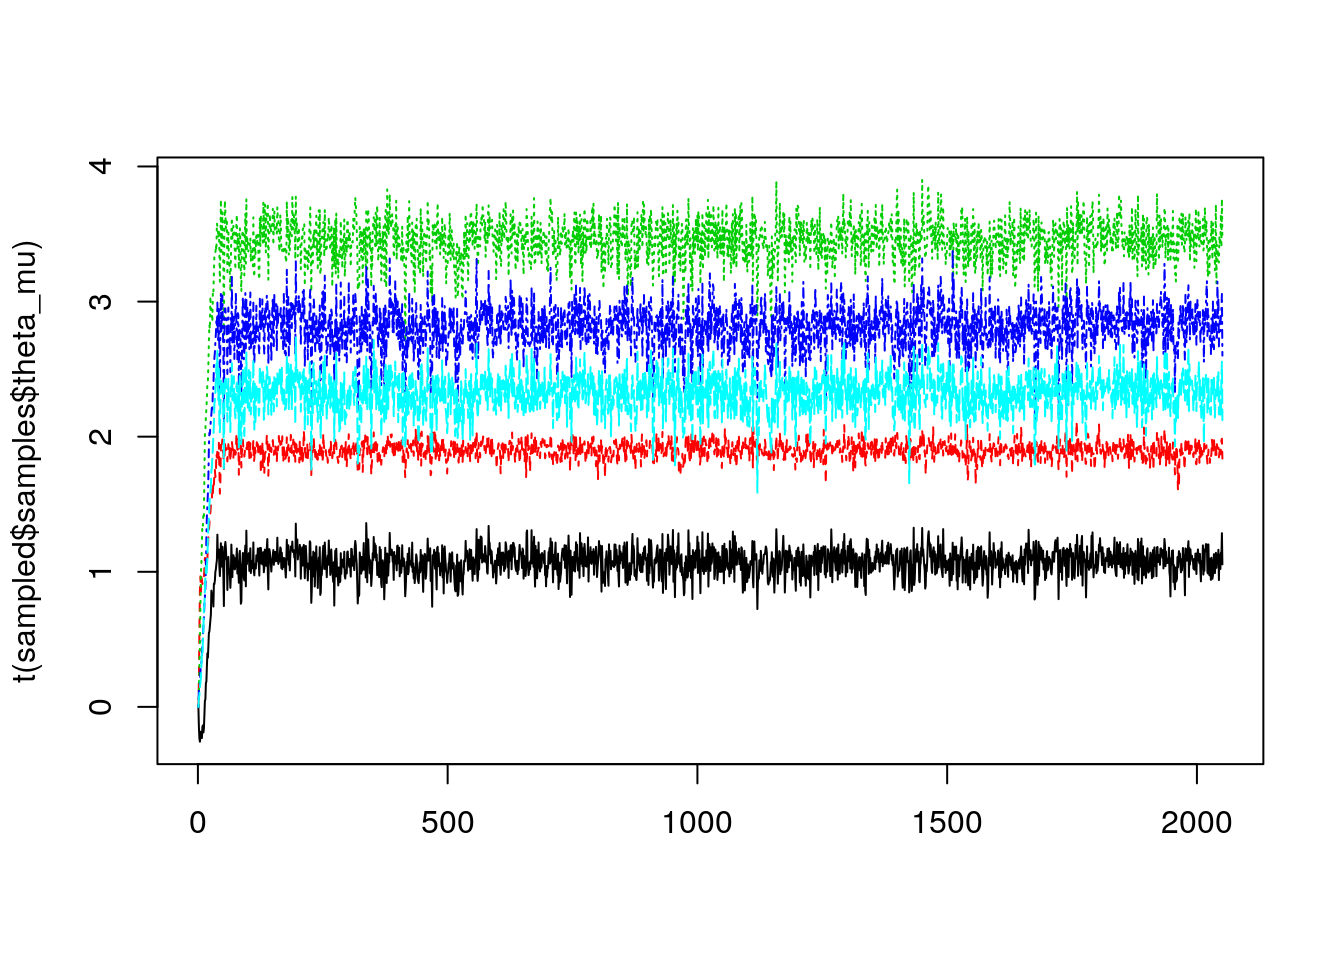
\includegraphics[width=1\linewidth]{bookdown-demo_files/figure-latex/parPlot-1} \caption{Posterior samples of parameters}\label{fig:parPlot}
\end{figure}

The second plot below (\ref{fig:subjLLPlot}) shows the likelihoods across iterations for each subject. Again we see that the likelihood values jump up after only a few iterations and then remain stable, with only slight movement.

\begin{figure}
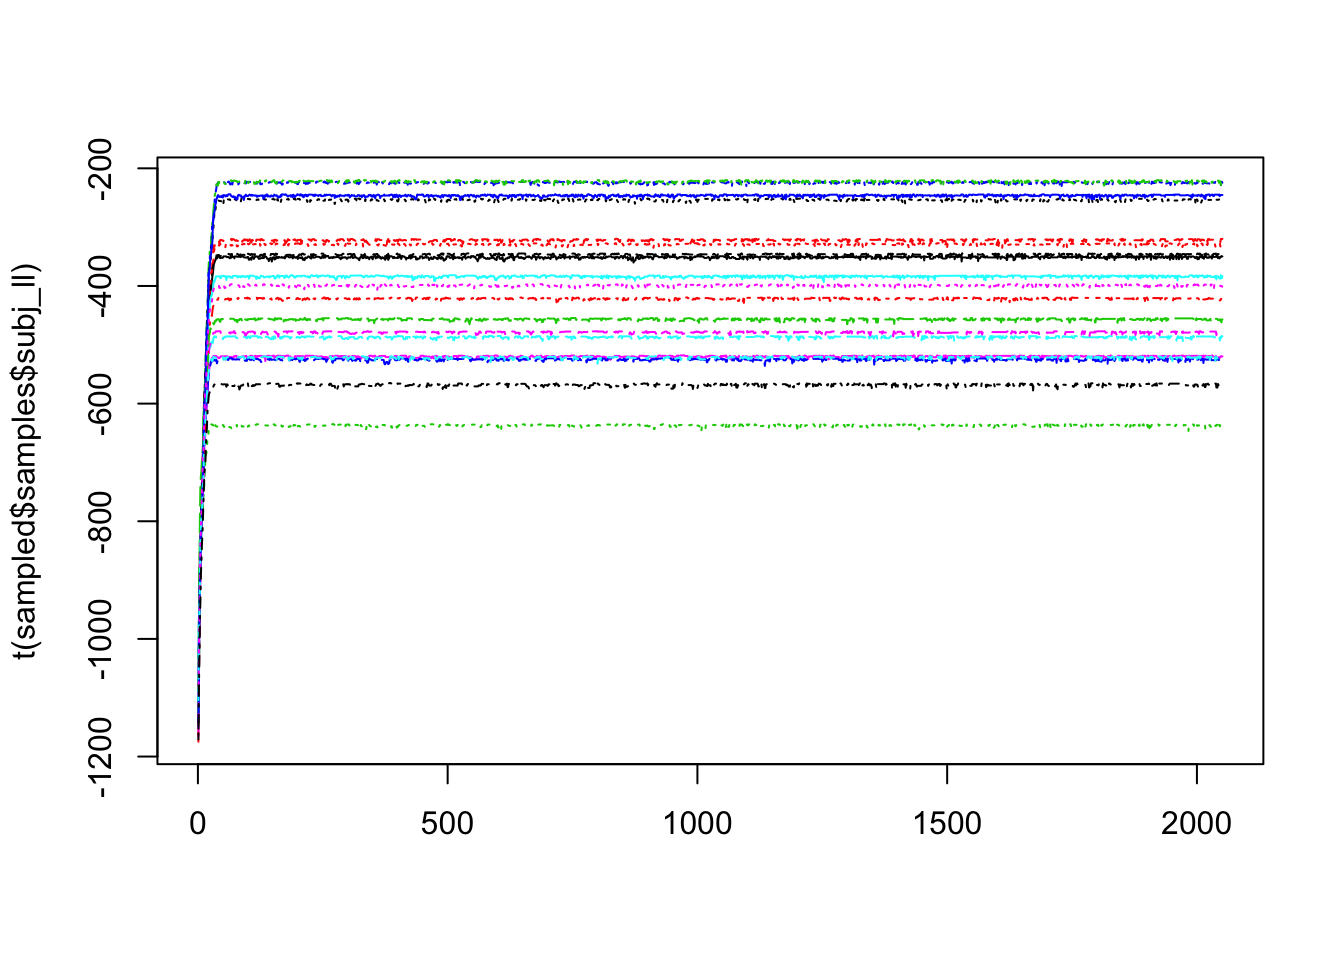
\includegraphics[width=1\linewidth]{bookdown-demo_files/figure-latex/subjLLPlot-1} \caption{Posterior samples of subject log likelihoods}\label{fig:subjLLPlot}
\end{figure}

\hypertarget{simulating-posterior-data}{%
\section{Simulating posterior data}\label{simulating-posterior-data}}

Now we'll cover the sample operation within the fast log likelihood function. We will use this on the full data set. The sample operation can be carried out in several ways (using rbinom etc). Please not that we do NOT recommend using this approach below and this should serve as an example only.

The \texttt{sample} process is similar to what we've covered above. We begin by assigning \texttt{NA}s to the response column to prepare it for simulated response data. We then consider a subset of the data, beginning with word condition and high-frequency \texttt{hf} word stimuli trials.

\begin{Shaded}
\begin{Highlighting}[]
  \ControlFlowTok{else}\NormalTok{\{}
\NormalTok{    data}\OperatorTok{$}\NormalTok{resp <-}\StringTok{ }\OtherTok{NA}
   \ControlFlowTok{for}\NormalTok{ (i }\ControlFlowTok{in} \DecValTok{1}\OperatorTok{:}\KeywordTok{nrow}\NormalTok{(data))\{}
      \ControlFlowTok{if}\NormalTok{ (data}\OperatorTok{$}\NormalTok{cond[i] }\OperatorTok{==}\StringTok{ "w"}\NormalTok{)\{}
        \ControlFlowTok{if}\NormalTok{ (data}\OperatorTok{$}\NormalTok{stim[i] }\OperatorTok{==}\StringTok{ "hf"}\NormalTok{)\{}
\end{Highlighting}
\end{Shaded}

We then take the criterion for the word condition i.e. \texttt{C.w}. To simulate a response given our parameters we use \texttt{rnorm} to pick a random value from a normal distribution with \texttt{mean\ =\ HF.d} (i.e.~high frequency word stimulus) and a SD of 1 and we test that value against the word criterion \texttt{C.w}. If the value is larger than \texttt{C.w}, the simulated response will be word otherwise, the simulated response will be non-word.

\begin{Shaded}
\begin{Highlighting}[]
\NormalTok{data}\OperatorTok{$}\NormalTok{resp[i] <-}\StringTok{ }\KeywordTok{ifelse}\NormalTok{(}\DataTypeTok{test =}\NormalTok{ (}\KeywordTok{rnorm}\NormalTok{(}\DecValTok{1}\NormalTok{, }\DataTypeTok{mean =}\NormalTok{ x[}\StringTok{"HF.d"}\NormalTok{], }
                                     \DataTypeTok{sd =} \DecValTok{1}\NormalTok{)) }\OperatorTok{>}\StringTok{ }\NormalTok{x[}\StringTok{"C.w"}\NormalTok{], }\StringTok{"word"}\NormalTok{, }\StringTok{"non-word"}\NormalTok{)}
\end{Highlighting}
\end{Shaded}

We repeat this process for each condition and stimulus combination as shown in the code block below.

\begin{Shaded}
\begin{Highlighting}[]
\NormalTok{\{ }\ControlFlowTok{else} \ControlFlowTok{if}\NormalTok{ (data}\OperatorTok{$}\NormalTok{stim[i] }\OperatorTok{==}\StringTok{ "lf"}\NormalTok{) \{}
\NormalTok{  data}\OperatorTok{$}\NormalTok{resp[i] <-}\StringTok{ }\KeywordTok{ifelse}\NormalTok{(}\DataTypeTok{test =}\NormalTok{ (}\KeywordTok{rnorm}\NormalTok{(}\DecValTok{1}\NormalTok{, }\DataTypeTok{mean =}\NormalTok{ x[}\StringTok{"LF.d"}\NormalTok{], }
                                       \DataTypeTok{sd =} \DecValTok{1}\NormalTok{)) }\OperatorTok{>}\StringTok{ }\NormalTok{x[}\StringTok{"C.w"}\NormalTok{], }\StringTok{"word"}\NormalTok{, }\StringTok{"non-word"}\NormalTok{)}
\NormalTok{  \} }\ControlFlowTok{else} \ControlFlowTok{if}\NormalTok{ (data}\OperatorTok{$}\NormalTok{stim[i] }\OperatorTok{==}\StringTok{ "vlf"}\NormalTok{) \{}
\NormalTok{    data}\OperatorTok{$}\NormalTok{resp[i] <-}\StringTok{ }\KeywordTok{ifelse}\NormalTok{(}\DataTypeTok{test =}\NormalTok{ (}\KeywordTok{rnorm}\NormalTok{(}\DecValTok{1}\NormalTok{, }\DataTypeTok{mean =}\NormalTok{ x[}\StringTok{"VLF.d"}\NormalTok{], }
                                         \DataTypeTok{sd =} \DecValTok{1}\NormalTok{)) }\OperatorTok{>}\StringTok{ }\NormalTok{x[}\StringTok{"C.w"}\NormalTok{], }\StringTok{"word"}\NormalTok{, }\StringTok{"non-word"}\NormalTok{)}
\NormalTok{    \} }\ControlFlowTok{else}\NormalTok{ \{}
\NormalTok{      data}\OperatorTok{$}\NormalTok{resp[i] <-}\StringTok{ }\KeywordTok{ifelse}\NormalTok{(}\DataTypeTok{test =}\NormalTok{ (}\KeywordTok{rnorm}\NormalTok{(}\DecValTok{1}\NormalTok{, }\DataTypeTok{mean =} \DecValTok{0}\NormalTok{, }
                                           \DataTypeTok{sd =} \DecValTok{1}\NormalTok{)) }\OperatorTok{>}\StringTok{ }\NormalTok{x[}\StringTok{"C.w"}\NormalTok{], }\StringTok{"word"}\NormalTok{, }\StringTok{"non-word"}\NormalTok{)}
\NormalTok{      \}}
\NormalTok{\} }\ControlFlowTok{else}\NormalTok{ \{}
  \ControlFlowTok{if}\NormalTok{ (data}\OperatorTok{$}\NormalTok{stim[i] }\OperatorTok{==}\StringTok{ "hf"}\NormalTok{) \{}
\NormalTok{    data}\OperatorTok{$}\NormalTok{resp[i] <-}\StringTok{ }\KeywordTok{ifelse}\NormalTok{(}\DataTypeTok{test =}\NormalTok{ (}\KeywordTok{rnorm}\NormalTok{(}\DecValTok{1}\NormalTok{, }\DataTypeTok{mean =}\NormalTok{ x[}\StringTok{"HF.d"}\NormalTok{], }
                                         \DataTypeTok{sd =} \DecValTok{1}\NormalTok{)) }\OperatorTok{>}\StringTok{ }\NormalTok{x[}\StringTok{"C.nw"}\NormalTok{], }\StringTok{"word"}\NormalTok{, }\StringTok{"non-word"}\NormalTok{)}
\NormalTok{    \} }\ControlFlowTok{else} \ControlFlowTok{if}\NormalTok{ (data}\OperatorTok{$}\NormalTok{stim[i] }\OperatorTok{==}\StringTok{ "lf"}\NormalTok{) \{}
\NormalTok{          data}\OperatorTok{$}\NormalTok{resp[i] <-}\StringTok{ }\KeywordTok{ifelse}\NormalTok{(}\DataTypeTok{test =}\NormalTok{ (}\KeywordTok{rnorm}\NormalTok{(}\DecValTok{1}\NormalTok{, }\DataTypeTok{mean =}\NormalTok{ x[}\StringTok{"LF.d"}\NormalTok{], }
                                               \DataTypeTok{sd =} \DecValTok{1}\NormalTok{)) }\OperatorTok{>}\StringTok{ }\NormalTok{x[}\StringTok{"C.nw"}\NormalTok{], }\StringTok{"word"}\NormalTok{, }\StringTok{"non-word"}\NormalTok{)}
\NormalTok{        \} }\ControlFlowTok{else} \ControlFlowTok{if}\NormalTok{ (data}\OperatorTok{$}\NormalTok{stim[i] }\OperatorTok{==}\StringTok{ "vlf"}\NormalTok{) \{}
\NormalTok{          data}\OperatorTok{$}\NormalTok{resp[i] <-}\StringTok{ }\KeywordTok{ifelse}\NormalTok{(}\DataTypeTok{test =}\NormalTok{ (}\KeywordTok{rnorm}\NormalTok{(}\DecValTok{1}\NormalTok{, }\DataTypeTok{mean =}\NormalTok{ x[}\StringTok{"VLF.d"}\NormalTok{], }
                                               \DataTypeTok{sd =} \DecValTok{1}\NormalTok{)) }\OperatorTok{>}\StringTok{ }\NormalTok{x[}\StringTok{"C.nw"}\NormalTok{], }\StringTok{"word"}\NormalTok{, }\StringTok{"non-word"}\NormalTok{)}
\NormalTok{        \} }\ControlFlowTok{else}\NormalTok{ \{}
\NormalTok{          data}\OperatorTok{$}\NormalTok{resp[i] <-}\StringTok{ }\KeywordTok{ifelse}\NormalTok{(}\DataTypeTok{test =}\NormalTok{ (}\KeywordTok{rnorm}\NormalTok{(}\DecValTok{1}\NormalTok{, }\DataTypeTok{mean =} \DecValTok{0}\NormalTok{, }
                                               \DataTypeTok{sd =} \DecValTok{1}\NormalTok{)) }\OperatorTok{>}\StringTok{ }\NormalTok{x[}\StringTok{"C.nw"}\NormalTok{], }\StringTok{"word"}\NormalTok{, }\StringTok{"non-word"}\NormalTok{)}
\NormalTok{          \}}
\NormalTok{        \}}
\end{Highlighting}
\end{Shaded}

Now we can run our simulation. Below is some code to achieve this.

\begin{Shaded}
\begin{Highlighting}[]
\NormalTok{n.posterior <-}\StringTok{ }\DecValTok{20} \CommentTok{# Number of samples from posterior distribution for each parameter.}
\NormalTok{pp.data <-}\StringTok{ }\KeywordTok{list}\NormalTok{()}
\NormalTok{S <-}\StringTok{ }\KeywordTok{unique}\NormalTok{(wgnmks2008}\OperatorTok{$}\NormalTok{subject)}
\NormalTok{data =}\StringTok{ }\KeywordTok{split}\NormalTok{(}\DataTypeTok{x =}\NormalTok{ wgnmks2008, }\DataTypeTok{f =}\NormalTok{ wgnmks2008}\OperatorTok{$}\NormalTok{subject)}
\ControlFlowTok{for}\NormalTok{ (s }\ControlFlowTok{in}\NormalTok{ S) \{}
  \KeywordTok{cat}\NormalTok{(s,}\StringTok{" "}\NormalTok{)}
\NormalTok{  iterations =}\StringTok{ }\KeywordTok{round}\NormalTok{(}\KeywordTok{seq}\NormalTok{(}\DataTypeTok{from =} \DecValTok{1051}\NormalTok{, }\DataTypeTok{to =}\NormalTok{ sampled}\OperatorTok{$}\NormalTok{samples}\OperatorTok{$}\NormalTok{idx, }\DataTypeTok{length.out =}\NormalTok{ n.posterior))}
  \ControlFlowTok{for}\NormalTok{ (i }\ControlFlowTok{in} \DecValTok{1}\OperatorTok{:}\KeywordTok{length}\NormalTok{(iterations)) \{}
\NormalTok{    x <-}\StringTok{ }\NormalTok{sampled}\OperatorTok{$}\NormalTok{samples}\OperatorTok{$}\NormalTok{alpha[, s, iterations[i]]}
    \KeywordTok{names}\NormalTok{(x) <-}\StringTok{ }\NormalTok{pars}
\NormalTok{    tmp <-}\StringTok{ }\KeywordTok{SDT_ll_fast}\NormalTok{(}\DataTypeTok{x =}\NormalTok{ x, }\DataTypeTok{data =}\NormalTok{ wgnmks2008[wgnmks2008}\OperatorTok{$}\NormalTok{subject }\OperatorTok{==}\StringTok{ }\NormalTok{s,], }\DataTypeTok{sample =} \OtherTok{TRUE}\NormalTok{)}
    \ControlFlowTok{if}\NormalTok{ (i }\OperatorTok{==}\StringTok{ }\DecValTok{1}\NormalTok{) \{}
\NormalTok{      pp.data[[s]] <-}\StringTok{ }\KeywordTok{cbind}\NormalTok{(i,tmp)}
\NormalTok{    \} }\ControlFlowTok{else}\NormalTok{ \{}
\NormalTok{      pp.data[[s]] <-}\StringTok{ }\KeywordTok{rbind}\NormalTok{(pp.data[[s]], }\KeywordTok{cbind}\NormalTok{(i, tmp))}
\NormalTok{    \}}
\NormalTok{  \}}
  
\NormalTok{\}}
\end{Highlighting}
\end{Shaded}

And now we can plot samples against the data.

\begin{figure}
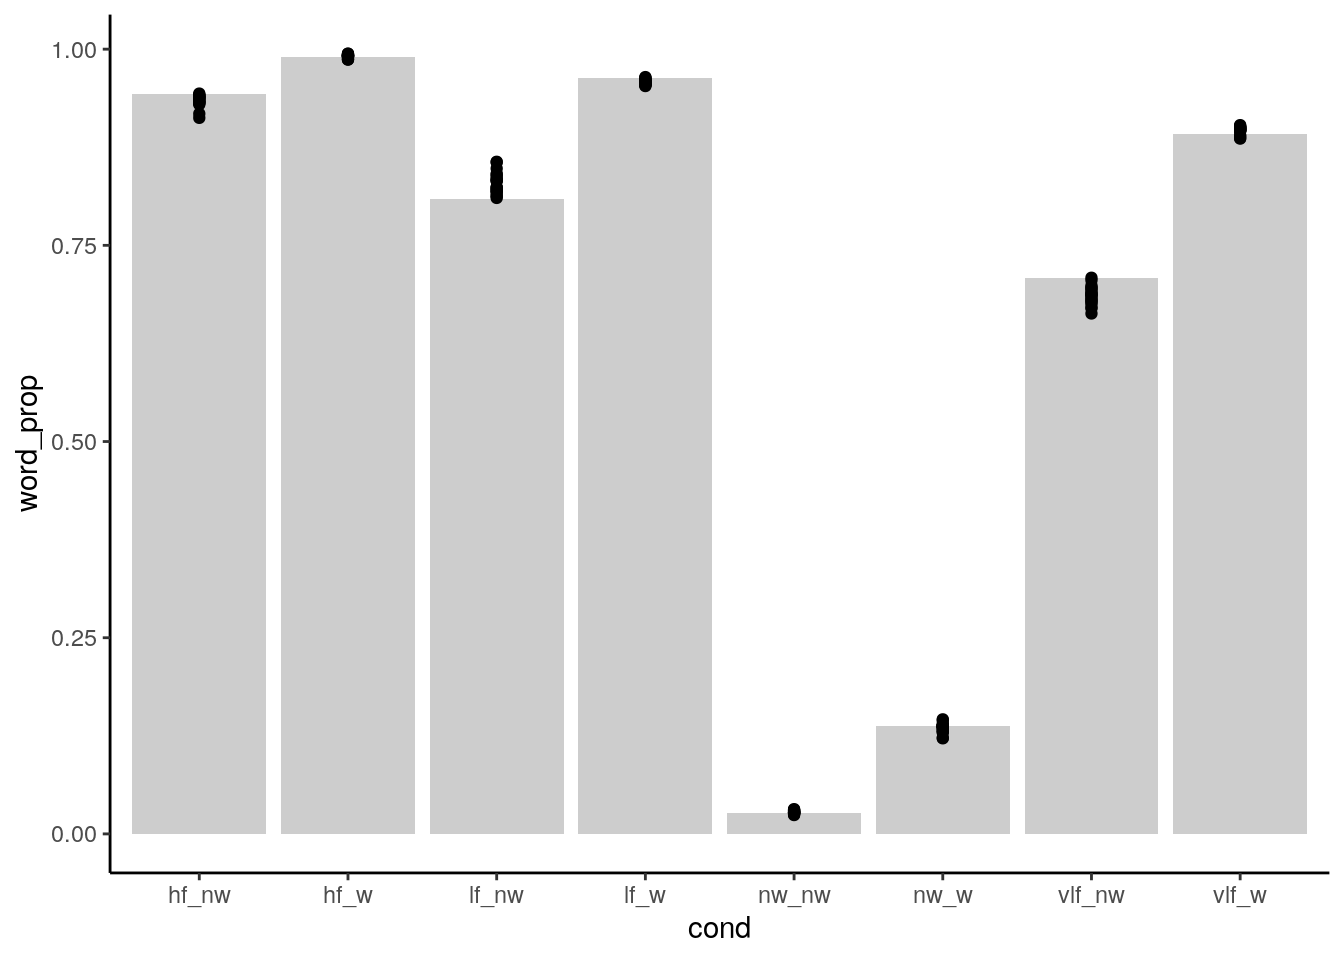
\includegraphics[width=1\linewidth]{bookdown-demo_files/figure-latex/part12graph-1} \caption{Appropriate figure caption HERE}\label{fig:part12graph}
\end{figure}

Figure \ref{fig:part12graph} shows 20 posterior draws (dots) plotted against the data (bars). The posterior draws are for each individual subject - shown here is the average proportion of word responses. Evidently, the model appears to fit the data well.

\#PMwG sampler and sequential sampling models

In this chapter we'll demonstrate how to use the PMwG sampler with a sequential sampling model; the Linear Ballistic Accumulator (LBA).
Please ensure the psamplers package is installed. We currently recommended installing psamplers via devtools.

\begin{Shaded}
\begin{Highlighting}[]
\CommentTok{# The samplers package will be on CRAN - this step will be removed.}
\KeywordTok{install_github}\NormalTok{(}\StringTok{'newcastlecl\textbackslash{}pmwg'}\NormalTok{)}
\end{Highlighting}
\end{Shaded}

\begin{Shaded}
\begin{Highlighting}[]
\KeywordTok{library}\NormalTok{(pmwg)}
\end{Highlighting}
\end{Shaded}

\hypertarget{description-of-forstmann-experiment}{%
\section{Description of Forstmann experiment}\label{description-of-forstmann-experiment}}

Forstmann et al looked at neural correlates of decision making under time pressure, with an aim to identify areas of the brain associated with speed-accuracy tradeoff. Imaging (fMRI) and behavioural data was collected; however, we will analyse behavioural data from the decision-making task only. In terms of modelling the data, Forstmann expected to find differences in thresholds (direction?) for each of the three speed-emphasis conditions. We have included the Forstmann et als data in the psamplers package as a data frame object named \texttt{forstmann}. The sampler requires a data frame with a \texttt{subject} column. The subject column data type can be a factor or numeric.

Table \ref{tab:forsthead10} shows the first ten trials from the Forstmann dataset. Participants \texttt{(n\ =\ 19)} were asked to indicate whether a cloud of dots in a random-dot kinematogram (RDK) moved to the left or the right of the screen. The IV was a within-subject, speed-accuracy manipulation where, before each trial began, pariticipants were instructed to make their choice accurately \texttt{(condition\ =\ 1)}, with urgency\texttt{(condition\ =\ 3)}or were presented with a neutral message \texttt{(condition\ =\ 2)}. Choice and response time data was collected. Choices were coded as correct \texttt{(correct\ =\ 2)} or incorrect \texttt{(correct\ =\ \ 1)} and response times \texttt{(rt)} were recorded in seconds. For more information about the design of the experiment please see \href{https://www.pnas.org/content/105/45/17538.short}{the original paper}.

\begin{table}

\caption{\label{tab:forsthead10}First 10 trials in Forstmann dataset. The `forstmann` dataset is an object/data frame }
\centering
\begin{tabular}[t]{l|r|l|l|l|r}
\hline
  & subject & condition & stim & resp & rt\\
\hline
1115 & 1 & 1 & 2 & 2 & 0.4319\\
\hline
1116 & 1 & 3 & 2 & 2 & 0.5015\\
\hline
1117 & 1 & 3 & 1 & 1 & 0.3104\\
\hline
1118 & 1 & 1 & 2 & 2 & 0.4809\\
\hline
1119 & 1 & 1 & 1 & 1 & 0.3415\\
\hline
1120 & 1 & 2 & 1 & 1 & 0.3465\\
\hline
1121 & 1 & 2 & 1 & 1 & 0.3572\\
\hline
1122 & 1 & 2 & 2 & 2 & 0.4042\\
\hline
1123 & 1 & 2 & 1 & 1 & 0.3866\\
\hline
1124 & 1 & 1 & 2 & 2 & 0.3683\\
\hline
\end{tabular}
\end{table}

\hypertarget{setting-up-the-sampler}{%
\section{Setting up the sampler}\label{setting-up-the-sampler}}

There are a number of preliminary steps we need to complete before running the sampler. Let's begin by defining the Linear Ballistic Accumulator (LBA) \citep{brown2008simplest} model parameters.

\begin{itemize}
\tightlist
\item
  \texttt{b} threshold parameter (the evidence required to make a response)
\item
  \texttt{v} is drift rate or average speed of evidence accumulation
\item
  \texttt{A} is the model's start point
\item
  \texttt{t0} is non-decision time.
\item
  Do we need to mention \texttt{sv} here? 
\end{itemize}

Now we know the LBA model parameters, we can create a vector of model parameter names, which we'll use in our log likelihood function. You can name this object as you wish; however, in our example, we will call it \texttt{pars}. The parameters you list in the \texttt{pars} vector must match the names and number of parameters you include in your log likelihood function.

\begin{Shaded}
\begin{Highlighting}[]
\NormalTok{pars <-}\StringTok{ }\KeywordTok{c}\NormalTok{(}\StringTok{"b1"}\NormalTok{, }\StringTok{"b2"}\NormalTok{, }\StringTok{"b3"}\NormalTok{, }\StringTok{"A"}\NormalTok{, }\StringTok{"v1"}\NormalTok{, }\StringTok{"v2"}\NormalTok{, }\StringTok{"t0"}\NormalTok{)}
\end{Highlighting}
\end{Shaded}

For the Forstmann dataset, we need three threshold parameters (\texttt{b1}, \texttt{b2}, and \texttt{b3} i.e.~one for each condition) because we assume that the participant responds to each condition with a different level of caution. We include two drift rate parameters: \texttt{v1} for the incorrect accumulator and \texttt{v2} for the correct accumulator, a start point parameter \texttt{A} and a non-decision time \texttt{t0} parameter. We've made a decision to set the \texttt{sv} to 1 to satisfy the scaling properties of the model, as such we haven't included the \texttt{sv} parameter in the \texttt{pars} vector - it is found in the LBA's likelihood function (see below).

Next we create a \texttt{priors} object; a list that contains two components Do we need to explain what priors are and why we do this?

\begin{itemize}
\tightlist
\item
  \texttt{theta\_mu} a vector containing the prior for model parameter means
\item
  \texttt{theta\_sig} the prior covariance matrix for model parameters.
\end{itemize}

\begin{Shaded}
\begin{Highlighting}[]
\NormalTok{priors <-}\StringTok{ }\KeywordTok{list}\NormalTok{(}\DataTypeTok{theta_mu =} \KeywordTok{rep}\NormalTok{(}\DecValTok{0}\NormalTok{, }\KeywordTok{length}\NormalTok{(pars)),}
  \DataTypeTok{theta_sig =} \KeywordTok{diag}\NormalTok{(}\KeywordTok{rep}\NormalTok{(}\DecValTok{1}\NormalTok{, }\KeywordTok{length}\NormalTok{(pars)))}
\NormalTok{)}
\end{Highlighting}
\end{Shaded}

The \texttt{priors} object in our example is initiated with zeros. Under what conditions would this priors object differ?

\hypertarget{writing-the-lba-log-likelihood-function}{%
\section{Writing the LBA Log-Likelihood Function}\label{writing-the-lba-log-likelihood-function}}

Now we have our parameter vector and priors object, we can write our log likelihood functions. Just as we did with the SDT example, we'll write a slow and a fast log likelihood function. The runtime difference is caused by calling the \texttt{dLBA} function line-by-line for the slow log likelihood and calling the \texttt{dLBA} function once for all the data in the fast log likelihood function. When writing a new log likelihood function, we suggest starting with a slow, line-by-line function for easier debugging.

The \texttt{lba\_loglike} function takes three arguments:

\begin{itemize}
\tightlist
\item
  \texttt{x} is a named parameter vector (e.g. \texttt{pars})
\item
  \texttt{data} is your data set (e.g.\texttt{forstmann})
\item
  \texttt{sample\ =\ FALSE} calculates a density function or \texttt{TRUE} generates a posterior, predictive sample that matches the shape of data.
\end{itemize}

The log-likelihood function requires three arguments:
- x: a vector of named parameter values.
- data: a data set (which must include a ``subject'' column)
- sample: to generate a posterior predictive sample that matches the shape of data (when set to TRUE)

The log likelihood function shown below includes functions from the \texttt{rtdists} package for generating data and estimating density.

Or you can write a log likelihood function as we have done with the LBA log likelihood function below. If you'd like to run through this example, it is best to copy the \texttt{lba\_loglike} function from the code block below rather than copying from the following separate code chunks, as some curly braces have been removed from code chunks.

\begin{Shaded}
\begin{Highlighting}[numbers=left,,]
\NormalTok{lba_loglike <-}\StringTok{ }\ControlFlowTok{function}\NormalTok{(x, data, }\DataTypeTok{sample =} \OtherTok{FALSE}\NormalTok{) \{}
\NormalTok{  x <-}\StringTok{ }\KeywordTok{exp}\NormalTok{(x)}
  \ControlFlowTok{if}\NormalTok{ (}\KeywordTok{any}\NormalTok{(data}\OperatorTok{$}\NormalTok{rt }\OperatorTok{<}\StringTok{ }\NormalTok{x[}\StringTok{"t0"}\NormalTok{])) \{}
    \KeywordTok{return}\NormalTok{(}\OperatorTok{-}\FloatTok{1e10}\NormalTok{)}
\NormalTok{  \}}

\NormalTok{  bs <-}\StringTok{ }\NormalTok{x[}\StringTok{"A"}\NormalTok{] }\OperatorTok{+}\StringTok{ }\NormalTok{x[}\KeywordTok{c}\NormalTok{(}\StringTok{"b1"}\NormalTok{, }\StringTok{"b2"}\NormalTok{, }\StringTok{"b3"}\NormalTok{)][data}\OperatorTok{$}\NormalTok{condition]}

  \ControlFlowTok{if}\NormalTok{ (sample) \{}
\NormalTok{    out <-}\StringTok{ }\NormalTok{rtdists}\OperatorTok{::}\KeywordTok{rLBA}\NormalTok{(}\DataTypeTok{n =} \KeywordTok{nrow}\NormalTok{(data),}
                         \DataTypeTok{A =}\NormalTok{ x[}\StringTok{"A"}\NormalTok{],}
                         \DataTypeTok{b =}\NormalTok{ bs,}
                         \DataTypeTok{t0 =}\NormalTok{ x[}\StringTok{"t0"}\NormalTok{],}
                         \DataTypeTok{mean_v =}\NormalTok{ x[}\KeywordTok{c}\NormalTok{(}\StringTok{"v1"}\NormalTok{, }\StringTok{"v2"}\NormalTok{)],}
                         \DataTypeTok{sd_v =} \KeywordTok{c}\NormalTok{(}\DecValTok{1}\NormalTok{, }\DecValTok{1}\NormalTok{),}
                         \DataTypeTok{distribution =} \StringTok{"norm"}\NormalTok{,}
                         \DataTypeTok{silent =} \OtherTok{TRUE}\NormalTok{)}
\NormalTok{  \} }\ControlFlowTok{else}\NormalTok{ \{}
\NormalTok{    out <-}\StringTok{ }\NormalTok{rtdists}\OperatorTok{::}\KeywordTok{dLBA}\NormalTok{(}\DataTypeTok{rt =}\NormalTok{ data}\OperatorTok{$}\NormalTok{rt,}
                         \DataTypeTok{response =}\NormalTok{ data}\OperatorTok{$}\NormalTok{correct,}
                         \DataTypeTok{A =}\NormalTok{ x[}\StringTok{"A"}\NormalTok{],}
                         \DataTypeTok{b =}\NormalTok{ bs,}
                         \DataTypeTok{t0 =}\NormalTok{ x[}\StringTok{"t0"}\NormalTok{],}
                         \DataTypeTok{mean_v =}\NormalTok{ x[}\KeywordTok{c}\NormalTok{(}\StringTok{"v1"}\NormalTok{, }\StringTok{"v2"}\NormalTok{)],}
                         \DataTypeTok{sd_v =} \KeywordTok{c}\NormalTok{(}\DecValTok{1}\NormalTok{, }\DecValTok{1}\NormalTok{),}
                         \DataTypeTok{distribution =} \StringTok{"norm"}\NormalTok{,}
                         \DataTypeTok{silent =} \OtherTok{TRUE}\NormalTok{)}
\NormalTok{    bad <-}\StringTok{ }\NormalTok{(out }\OperatorTok{<}\StringTok{ }\FloatTok{1e-10}\NormalTok{) }\OperatorTok{|}\StringTok{ }\NormalTok{(}\OperatorTok{!}\KeywordTok{is.finite}\NormalTok{(out))}
\NormalTok{    out[bad] <-}\StringTok{ }\FloatTok{1e-10}
\NormalTok{    out <-}\StringTok{ }\KeywordTok{sum}\NormalTok{(}\KeywordTok{log}\NormalTok{(out))}
\NormalTok{  \}}
\NormalTok{  out}
\NormalTok{\}}
\end{Highlighting}
\end{Shaded}

The first line in the \texttt{lba\_loglike} function (Line 2 below) takes the exponent of the parameter values to move all parameter values to the real line. The purpose of this is to\ldots{}..
Line 3 and 4 then checks RTs are faster than the non-decision time parameter, and zero those RTs that are faster than non-decision time.

\begin{Shaded}
\begin{Highlighting}[numbers=left,,]
\NormalTok{lba_loglike <-}\StringTok{ }\ControlFlowTok{function}\NormalTok{(x, data, }\DataTypeTok{sample =} \OtherTok{FALSE}\NormalTok{) \{}
\NormalTok{  x <-}\StringTok{ }\KeywordTok{exp}\NormalTok{(x) }
  \ControlFlowTok{if}\NormalTok{ (}\KeywordTok{any}\NormalTok{(data}\OperatorTok{$}\NormalTok{rt }\OperatorTok{<}\StringTok{ }\NormalTok{x[}\StringTok{"t0"}\NormalTok{])) \{}
    \KeywordTok{return}\NormalTok{(}\OperatorTok{-}\FloatTok{1e10}\NormalTok{)}
\NormalTok{  \}}
\end{Highlighting}
\end{Shaded}

Next (Line 7) we create a vector containing threshold parameters for each row in the data set that takes into account the condition and adds the start point value. We add the start point parameter \texttt{A} value to each threshold parameter so that threshold is greater than the start point value.

\begin{Shaded}
\begin{Highlighting}[numbers=left,,firstnumber=7,]
\NormalTok{  bs <-}\StringTok{ }\NormalTok{x[}\StringTok{"A"}\NormalTok{] }\OperatorTok{+}\StringTok{ }\NormalTok{x[}\KeywordTok{c}\NormalTok{(}\StringTok{"b1"}\NormalTok{, }\StringTok{"b2"}\NormalTok{, }\StringTok{"b3"}\NormalTok{)][data}\OperatorTok{$}\NormalTok{condition]}
\end{Highlighting}
\end{Shaded}

The \texttt{if\ else} statement below (Line 9-32) does one of two things: \texttt{if\ (sample)} calculates the posterior predictive data and the \texttt{else} statement calculates the density function. Toward the end of the \texttt{else} statment (line 28) we take all implausible likelihood values, assign them to the \texttt{bad} object and set them to zero. The final line in the \texttt{else} statement takes the log of all likelihood values, sums them and then assigns the model's log likelihood value to the \texttt{out} variable.

\begin{Shaded}
\begin{Highlighting}[numbers=left,,firstnumber=9,]
  \ControlFlowTok{if}\NormalTok{ (sample) \{}
\NormalTok{    out <-}\StringTok{ }\NormalTok{rtdists}\OperatorTok{::}\KeywordTok{rLBA}\NormalTok{(}\DataTypeTok{n =} \KeywordTok{nrow}\NormalTok{(data),}
                         \DataTypeTok{A =}\NormalTok{ x[}\StringTok{"A"}\NormalTok{],}
                         \DataTypeTok{b =}\NormalTok{ bs,}
                         \DataTypeTok{t0 =}\NormalTok{ x[}\StringTok{"t0"}\NormalTok{],}
                         \DataTypeTok{mean_v =}\NormalTok{ x[}\KeywordTok{c}\NormalTok{(}\StringTok{"v1"}\NormalTok{, }\StringTok{"v2"}\NormalTok{)],}
                         \DataTypeTok{sd_v =} \KeywordTok{c}\NormalTok{(}\DecValTok{1}\NormalTok{, }\DecValTok{1}\NormalTok{),}
                         \DataTypeTok{distribution =} \StringTok{"norm"}\NormalTok{,}
                         \DataTypeTok{silent =} \OtherTok{TRUE}\NormalTok{)}
\NormalTok{  \} }\ControlFlowTok{else}\NormalTok{ \{}
\NormalTok{    out <-}\StringTok{ }\NormalTok{rtdists}\OperatorTok{::}\KeywordTok{dLBA}\NormalTok{(}\DataTypeTok{rt =}\NormalTok{ data}\OperatorTok{$}\NormalTok{rt,}
                         \DataTypeTok{response =}\NormalTok{ data}\OperatorTok{$}\NormalTok{correct,}
                         \DataTypeTok{A =}\NormalTok{ x[}\StringTok{"A"}\NormalTok{],}
                         \DataTypeTok{b =}\NormalTok{ bs,}
                         \DataTypeTok{t0 =}\NormalTok{ x[}\StringTok{"t0"}\NormalTok{],}
                         \DataTypeTok{mean_v =}\NormalTok{ x[}\KeywordTok{c}\NormalTok{(}\StringTok{"v1"}\NormalTok{, }\StringTok{"v2"}\NormalTok{)],}
                         \DataTypeTok{sd_v =} \KeywordTok{c}\NormalTok{(}\DecValTok{1}\NormalTok{, }\DecValTok{1}\NormalTok{),}
                         \DataTypeTok{distribution =} \StringTok{"norm"}\NormalTok{,}
                         \DataTypeTok{silent =} \OtherTok{TRUE}\NormalTok{)}
\NormalTok{    bad <-}\StringTok{ }\NormalTok{(out }\OperatorTok{<}\StringTok{ }\FloatTok{1e-10}\NormalTok{) }\OperatorTok{|}\StringTok{ }\NormalTok{(}\OperatorTok{!}\KeywordTok{is.finite}\NormalTok{(out))}
\NormalTok{    out[bad] <-}\StringTok{ }\FloatTok{1e-10}
\NormalTok{    out <-}\StringTok{ }\KeywordTok{sum}\NormalTok{(}\KeywordTok{log}\NormalTok{(out))}
\NormalTok{  \}}
\NormalTok{  out}
\end{Highlighting}
\end{Shaded}

The next step is to include your log likelihood function. This must be called before you create the sampler object in the following step. You can load your log likelihood function from an external script:

\begin{Shaded}
\begin{Highlighting}[]
\KeywordTok{source}\NormalTok{(}\DataTypeTok{file =} \StringTok{"yourLogLikelihoodFile.R"}\NormalTok{)}
\end{Highlighting}
\end{Shaded}

Once you've setup your parameters, priors and your log likelihood function, the next step is to initialise the \texttt{sampler} object.

\begin{Shaded}
\begin{Highlighting}[]
\NormalTok{sampler <-}\StringTok{ }\KeywordTok{pmwgs}\NormalTok{(}
  \DataTypeTok{data =}\NormalTok{ forstmann,}
  \DataTypeTok{pars =}\NormalTok{ pars,}
  \DataTypeTok{prior =}\NormalTok{ priors,}
  \DataTypeTok{ll_func =}\NormalTok{ lba_loglike}
\NormalTok{)}
\end{Highlighting}
\end{Shaded}

The \texttt{pmwgs} function takes a set of arguments (listed below) and returns a list containing the required components for performing the particle metropolis within Gibbs steps.

\begin{itemize}
\tightlist
\item
  \texttt{data\ =} your data - a data frame (e.g.\texttt{forstmann}) with a column for participants called \texttt{subject}
\item
  \texttt{pars\ =} the model parameters to be used (e.g.\texttt{pars})
\item
  \texttt{prior\ =} the priors to be used (e.g.\texttt{priors})
\item
  \texttt{ll\_func\ =} name of log likelihood function you've sourced above (e.g.\texttt{lba\_loglike})
\end{itemize}

\hypertarget{start-points}{%
\subsection{Model start points}\label{start-points}}

You have the option to set model start points. We have specified sensible start points for the Forstmann dataset. If you chose not to specify start points, the sampler will randomly sample points from the prior distribution.

\begin{Shaded}
\begin{Highlighting}[]
\NormalTok{start_points <-}\StringTok{ }\KeywordTok{list}\NormalTok{(}
  \DataTypeTok{mu =} \KeywordTok{c}\NormalTok{(.}\DecValTok{2}\NormalTok{, }\FloatTok{.2}\NormalTok{, }\FloatTok{.2}\NormalTok{, }\FloatTok{.4}\NormalTok{, }\FloatTok{.3}\NormalTok{, }\FloatTok{1.3}\NormalTok{, }\DecValTok{-2}\NormalTok{),}
  \DataTypeTok{sig2 =} \KeywordTok{diag}\NormalTok{(}\KeywordTok{rep}\NormalTok{(.}\DecValTok{01}\NormalTok{, }\KeywordTok{length}\NormalTok{(pars)))}
\NormalTok{)}
\end{Highlighting}
\end{Shaded}

The \texttt{start\_points} object contains two vectors:

\begin{itemize}
\tightlist
\item
  \texttt{mu} a vector of start points for the mu of each model parameter
\item
  \texttt{sig2} vector containing the start points of the covariance matrix of covariance between model parameters.
\end{itemize}

\hypertarget{run-sampler}{%
\subsection{Running the sampler}\label{run-sampler}}

Okay - now we are ready to run the sampler.

\begin{Shaded}
\begin{Highlighting}[]
\NormalTok{sampler <-}\StringTok{ }\KeywordTok{init}\NormalTok{(sampler, }\DataTypeTok{theta_mu =}\NormalTok{ start_points}\OperatorTok{$}\NormalTok{mu,}
                \DataTypeTok{theta_sig =}\NormalTok{ start_points}\OperatorTok{$}\NormalTok{sig2)}
\end{Highlighting}
\end{Shaded}

Here we are using the \texttt{init} function to generate initial start points for the random effects and storing them in the \texttt{sampler} object. First we pass the \texttt{sampler} object from above that includes our data, parameters, priors and log likelihood function. If we decided to specify our own start points (as above), we would include the \texttt{theta\_mu} and \texttt{theta\_sig} arguments.

Now we can run the sampler using the \texttt{run\_stage} function. The \texttt{run\_stage} function takes four arguments:

\begin{itemize}
\tightlist
\item
  \texttt{x} the \texttt{sampler} object including parameters
\item
  \texttt{stage\ =} the sampling stage (e.g. \texttt{"burn"}, \texttt{"adapt"} or \texttt{"sample"})
\item
  \texttt{iter\ =} is the number of iterations for the sampling stage
\item
  \texttt{particles\ =} is the number of particles generated on each iteration
\end{itemize}

It is optional to include the \texttt{iter\ =} and \texttt{particles\ =} arguments. If these are not included, \texttt{iter} and \texttt{particles} default to 1000. The number of iterations you choose for your burn in stage is similar to choices made when running deMCMC, however, this varies depending on the time the model takes to reach the `real' posterior space.

First we run our burn in stage by setting \texttt{stage\ =} to \texttt{"burn"}. Here we have set iterations to be 500, which may take some time.

\begin{Shaded}
\begin{Highlighting}[]
\NormalTok{burned <-}\StringTok{ }\KeywordTok{run_stage}\NormalTok{(sampler, }\DataTypeTok{stage =} \StringTok{"burn"}\NormalTok{, }\DataTypeTok{iter =} \DecValTok{500}\NormalTok{, }\DataTypeTok{particles =} \DecValTok{1000}\NormalTok{)}
\end{Highlighting}
\end{Shaded}

Now we run our adaptation stage by setting \texttt{stage\ =\ "adapt"} Because we have not specified number of iterations or particles, the sampler will use the default value of 1000 for each of these arguments. N.B. The sampler will quit adaptation stage after 20 unique values have been accepted for each subject. This means adaptation may not use all 1000 iterations.

\begin{Shaded}
\begin{Highlighting}[]
\NormalTok{adapted <-}\StringTok{ }\KeywordTok{run_stage}\NormalTok{(burned, }\DataTypeTok{stage =} \StringTok{"adapt"}\NormalTok{)}
\end{Highlighting}
\end{Shaded}

At the start of the \texttt{sampled} stage, the sampler object will create a `proposal' distribution for each subject's random effects using a conditional multi-variate normal. This proposal distribution is then used to efficiently generate new particles for each subject which means we can reduce the number of particles on each iteration whilst still achieving acceptance rates.

\begin{Shaded}
\begin{Highlighting}[]
\NormalTok{sampled <-}\StringTok{ }\KeywordTok{run_stage}\NormalTok{(adapted, }\DataTypeTok{stage =} \StringTok{"sample"}\NormalTok{, }\DataTypeTok{iter =} \DecValTok{100}\NormalTok{, }\DataTypeTok{particles =} \DecValTok{100}\NormalTok{)}
\end{Highlighting}
\end{Shaded}

\hypertarget{example-2---single-threshold-parameter}{%
\chapter{Example 2 - Single threshold parameter}\label{example-2---single-threshold-parameter}}

In this second example, we will use a single \texttt{b} threshold parameter (the evidence required to make a response).
Altering the code/model is simple. First, update your parameter object (e.g.\texttt{pars}) by including a single \texttt{b} threshold parameter:

\begin{Shaded}
\begin{Highlighting}[]
\NormalTok{pars <-}\StringTok{ }\KeywordTok{c}\NormalTok{(}\StringTok{"b"}\NormalTok{, }\StringTok{"A"}\NormalTok{, }\StringTok{"v1"}\NormalTok{, }\StringTok{"v2"}\NormalTok{, }\StringTok{"t0"}\NormalTok{)}
\end{Highlighting}
\end{Shaded}

The \texttt{priors} object will update based on the length of your parameter object. Remove this?

\begin{Shaded}
\begin{Highlighting}[]
\NormalTok{priors <-}\StringTok{ }\KeywordTok{list}\NormalTok{(}\DataTypeTok{theta_mu =} \KeywordTok{rep}\NormalTok{(}\DecValTok{0}\NormalTok{, }\KeywordTok{length}\NormalTok{(pars)),}
  \DataTypeTok{theta_sig =} \KeywordTok{diag}\NormalTok{(}\KeywordTok{rep}\NormalTok{(}\DecValTok{1}\NormalTok{, }\KeywordTok{length}\NormalTok{(pars)))}
\NormalTok{)}
\end{Highlighting}
\end{Shaded}

The next step is to modify your log likelihood function by updating the threshold parameter vector (\texttt{bs}) so that the name and number of threshold parameters (\texttt{b}) matches the name and number of threshold parameters you've specified in your \texttt{pars} vector. In this case, we require a single \texttt{b} parameter.

\begin{Shaded}
\begin{Highlighting}[]
\NormalTok{  bs <-}\StringTok{ }\NormalTok{x[}\StringTok{"A"}\NormalTok{] }\OperatorTok{+}\StringTok{ }\NormalTok{x[}\StringTok{"b"}\NormalTok{][data}\OperatorTok{$}\NormalTok{condition]}
\end{Highlighting}
\end{Shaded}

The subsequent lines of code in the log likelihood function remain unchanged.

As mentioned in \protect\hyperlink{start-points}{example 1}, you may set model start points. It is important to provide the same number of values for \texttt{mu} as the number of parameters you've set in your \texttt{pars} vector.

\begin{Shaded}
\begin{Highlighting}[]
\NormalTok{start_points <-}\StringTok{ }\KeywordTok{list}\NormalTok{(}
  \DataTypeTok{mu =} \KeywordTok{c}\NormalTok{(.}\DecValTok{2}\NormalTok{,.}\DecValTok{4}\NormalTok{, }\FloatTok{.3}\NormalTok{, }\FloatTok{1.3}\NormalTok{, }\DecValTok{-2}\NormalTok{), }\CommentTok{# We have set five parameter start points here, }
                              \CommentTok{# matching the number of parameters in the pars vector.}
  \DataTypeTok{sig2 =} \KeywordTok{diag}\NormalTok{(}\KeywordTok{rep}\NormalTok{(.}\DecValTok{01}\NormalTok{, }\KeywordTok{length}\NormalTok{(pars)))}
\NormalTok{)}
\end{Highlighting}
\end{Shaded}

And now you're ready to run the sampler as outlined in \protect\hyperlink{run-sampler}{example 1}.

\hypertarget{example-3---wagenmakers-2008-experiment-2}{%
\chapter{Example 3 - Wagenmakers (2008) Experiment 2}\label{example-3---wagenmakers-2008-experiment-2}}

See iSquared paper eperiment 2

\hypertarget{common-problems-better-name-required-troubleshooting-page}{%
\chapter{Common Problems (Better name required) Troubleshooting page}\label{common-problems-better-name-required-troubleshooting-page}}

\hypertarget{how-to-write-a-log-likelihood-function}{%
\section{How to write a log likelihood function}\label{how-to-write-a-log-likelihood-function}}

\begin{itemize}
\tightlist
\item
  What key elements are required in a log likelihood function to be used in the sampler
\item
  Show comparison times for slow LL and fast LL
\item
  Check list for commmon errors - brief list check this, check that etc.
\end{itemize}

\hypertarget{writing-your-log-likelihood-function-tips-errors-and-check-list}{%
\subsection{Writing your log likelihood function: Tips, errors and check list}\label{writing-your-log-likelihood-function-tips-errors-and-check-list}}

1. The parameter specified does not exist

The parameter name is not specified to be estimated i.e.~it is not in the parameter names argument or it is misspelled. Make sure \texttt{pars} vector contains the same parameter names you have included in your log likelihood function and it is the same length. Do not rely on the log likelihood function to throw an error in this case.
(e.g.\texttt{x{[}‘b’{]}})

2. All non-continuous data frame variables must be a \texttt{factor}.

Data frame variables should be \href{https://www.rdocumentation.org/packages/base/versions/3.6.2/topics/factor}{\texttt{factors}} unless the variable is a continuous variable e.g.~response time.
If you pass \href{https://www.rdocumentation.org/packages/base/versions/3.6.2/topics/character}{\texttt{character}} variables to \texttt{if} statements and/or \texttt{for} loops in your log likelihood function, errors will not occur, however, your log likelihood estimate will be incorrect. For example,
avoid using character strings like \texttt{data\$condition\ ==\ “easy”}. If you must use a character string, be sure to convert the string to a factor with \texttt{as.factor}.

3. Spelling errors or mismatched column name references

Correctly reference data frame column names in your log likelihood function e.g. \texttt{data\$RT} != \texttt{data\$rt}.

4. When initialising a vector of parameter values - values are not filling in properly

E.g. When a vector for b for all the values across the data set to be used, but there are NAs filling it somewhere.

5. Make sure operations are done on the right scale.

6. Data frame variables are scaled appropriately for the model

Check your variables are correctly scaled and in the correct units. For example, with the LBA, response times must be in seconds rather than milliseconds.

7. The log likelihood is printed/outputted at the end of function

Make sure your log likelihood function prints an estimate at the end of the function and the estimate is correctly obtained e.g.~sum the log likelihood estimates for all trials/rows.

8. Sampling error occurs

When sampling, the generated columns are not outputted

9. When executing functions row by row (i.e.~trial-wise), index MUST be included

If writing a trial-wise/row-wise function (e.g. \texttt{if} statement, \texttt{for} loop), index \texttt{i} must be specified.

\begin{Shaded}
\begin{Highlighting}[]
\ControlFlowTok{if}\NormalTok{ (data}\OperatorTok{$}\NormalTok{condition }\OperatorTok{==}\StringTok{ }\NormalTok{“easy”)     }\CommentTok{# Incorrect reference when iterating over variable}
\ControlFlowTok{if}\NormalTok{ (data}\OperatorTok{$}\NormalTok{condition[i] }\OperatorTok{==}\StringTok{ }\NormalTok{“easy”)  }\CommentTok{# Include i index}
\end{Highlighting}
\end{Shaded}

10. Changing parameter values changes the log likelihood estimate

A simple check to run on your log likelihood function is to modify your parameter values and observe the change to log likelihood estimate. Then check if changing parameter values which rely on conditions actually change the log likelihood estimate.

11. Make sure you have the latest version of the PMwG Samplers package

checkVersion(``psamplers'')

\hypertarget{non-rtchoice-example}{%
\chapter{Non RT/Choice example}\label{non-rtchoice-example}}

\bibliography{book.bib,packages.bib}

\end{document}
